\documentclass[a4paper, 12pt]{report}
\usepackage{cmap}
\usepackage{amssymb}
\usepackage{amsmath}
\usepackage{graphicx}
\usepackage{amsthm}
\usepackage{upgreek}
\usepackage{setspace}
\usepackage[T2A]{fontenc}
\usepackage[utf8]{inputenc}
\usepackage[normalem]{ulem}
\usepackage{mathtext} % русские буквы в формулах
\usepackage[left=2cm,right=2cm, top=2cm,bottom=2cm,bindingoffset=0cm]{geometry}
\usepackage[english,russian]{babel}
\usepackage[unicode]{hyperref}
\newenvironment{Proof} % имя окружения
{\par\noindent{$\blacklozenge$}} % команды для \begin
{\hfill$\scriptstyle\boxtimes$}
\newcommand{\grad}{\operatorname{grad}}
\newcommand{\Sp}{\operatorname{Sp}}
\newcommand{\Rm}{\mathbb{R}}
\newcommand{\Cm}{\mathbb{C}}
\newcommand{\Z}{\mathbb{Z}}
\newcommand{\I}{\mathbb{I}}
\newcommand{\N}{\mathbb{N}}
\newcommand{\rank}{\operatorname{rank}}
\newcommand{\Ra}{\Rightarrow}
\newcommand{\ra}{\rightarrow}
\newcommand{\FI}{\Phi}
\renewcommand{\leq}{\leqslant}
\renewcommand{\geq}{\geqslant}
\renewcommand{\alpha}{\upalpha}
\renewcommand{\beta}{\upbeta}
\renewcommand{\gamma}{\upgamma}
\renewcommand{\delta}{\updelta}
\renewcommand{\varphi}{\upvarphi}
\renewcommand{\tau}{\uptau}
\renewcommand{\lambda}{\uplambda}
\renewcommand{\psi}{\uppsi}
\renewcommand{\mu}{\upmu}
\renewcommand{\omega}{\upomega}
\renewcommand{\d}{\partial}
\renewcommand{\xi}{\upxi}
\renewcommand{\epsilon}{\upvarepsilon}
\newcommand{\intx}{\int\limits_{x_0}^x}
\newcommand\Norm[1]{\left\| #1 \right\|}
\newcommand{\Ln}{L_n = D^n + a_{n-1}D^{n-1} + \ldots + a_1D + a_0D^0}
\newcommand{\KFunc}{\int\limits_{t_0}^{t}\varphi_{n-1}(t-\uptau)f(\uptau)d\uptau}
\newcommand{\sumk}{\sum\limits_{k=0}^\infty}
\newcommand{\sumi}{\sum\limits_{i=0}^\infty}
\newtheorem*{theorem}{Теорема}
\newtheorem*{cor}{Следствие}
\newtheorem*{lem}{Лемма}
\title{\textbf{\Huge{Вычислительные методы алгебры}}\\Конспект по 3 курсу 
	специальности «прикладная математика»\\(лектор А. М. Будник)}
\date{}
\begin{document}
	\maketitle
	\tableofcontents{}
	\newpage
	\chapter{Введение.}
	\section{Математическое моделирование и вычислительные эксперименты.}
	$\bullet$ \textit{\textbf{Математическое моделирование} --- описание реальных явлений, процессов и объектов с помощью математических уравнений.}\\\\
	$\bullet$ \textit{\textbf{Вычислительный эксперимент} --- исследование естественных научных проблем средствами научной математики.}
	\begin{center}
		Схема вычислительного эксперимента
	\end{center}
	$$
\includegraphics[scale=0.6]{img1.png}$$
	В основе вычислительного эксперимента лежит решение уравнений математической модели численными методами. Под численными методами понимаются методы, работающие с приближенными данными.
	\section{Структура погрешности. Корректность.}
	Формально любую задачу можно определить следующим образом: если требуется определить некоторую величину $y$ по величине $x$, то символически задачу можно записать в виде $$y = A(x),$$ где $A$ --- некоторый оператор, действующий на величину $x$, а $y$ и $x$ --- числа, совокупности чисел, функции и так далее. Если оператор $A$ настолько сложный, что решение не удается явно выписать, то задачу решаем приближенно с помощью любого метода. При этой замене возникает погрешность.\\\\
	Причины возникновения погрешностей в решении задач:
	\begin{enumerate}
		\item математическое описание неточное;
		\item исходные данные заданы приближенно;
		\item метод не является точным;
		\item при вводе данных, выполнении математических операций и выводе производится округление из-за ограниченности расчетной сетки.
	\end{enumerate}
	Запишем погрешности, соответствующие причинам:
	\begin{enumerate}
		\item погрешность математической модели;
		\item неустранимая погрешность;
		\item погрешность метода;
		\item вычислительная погрешность.
	\end{enumerate}
	$\bullet$ \textit{Задача $y = A(x)$ называется \textbf{корректно поставленной}, если} \begin{enumerate}
		\item $\forall$ \textit{входных данных $\exists !$ решение} $y$;
		\item \textit{решение $y$ устойчиво по входным данным.}
	\end{enumerate}
	$\bullet$ \textit{Под \textbf{устойчивостью решения} $y$ по входным данным $x$ понимается непрерывная зависимость погрешности $\Delta x$ решения от погрешности $\Delta y$ входных данных (то есть если $\Delta x \to 0$, то $\Delta y \to 0$).}\\\\
	$\bullet$ \textit{При невыполнении хотя бы одного из этих условий задача называется \textbf{некорректной}.}
	\section{Элементы теории погрешностей.}
	Пусть $x$ --- точное, а $x^*$ --- приближенное значение некоторой величины. Тогда число $\epsilon = x - x^*$ --- погрешность приближенного значения $x^*$.\\\\
	Модуль величины погрешности оценивается $$|x-x^*| = |\epsilon| \leq \Delta (x^*),$$ где $\Delta(x^*)$ --- \textbf{абсолютная погрешность}.\\\\
	В свою очередь, $$\Big|\dfrac{x-x^*}{x^*} \Big| = \Big| \dfrac{\epsilon}{x^*}\Big| \leq \dfrac{\Delta(x^*)}{|x^*|} = \delta(x^*),$$ где $\delta(x^*)$ --- \textbf{относительная погрешность}.\\\\
	Основная задача теории погрешностей --- указание области неопределенности результатов. \\\\Рассмотрим задачу теории погрешностей. Пусть имеется функция $$y = f(x_1, x_2,\ldots, x_n).$$ \textbf{Прямая задача теории погрешностей} заключается в определении абсолютной погрешности вычисления функции по абсолютной погрешности определения аргументов.
	Обозначим $$x^* = (x_1^*, x_2^*, \ldots, x_n^*)$$ --- приближенное значение аргументов функции $f$, для которой известны $\Delta(x_i^*)$, $i = \overline{1,n}$; $$x = (x_1, x_2\ldots, x_n)$$ --- точное значение аргументов. Воспользуемся формулой конечных приращений Лагранжа $$f(x) = f(x^*) + \sum_{i=1}^{n} \dfrac{\partial f (x^* + \theta(x-x^*))}{\partial x_i}\cdot (x_i - x_i^*), \quad 0 < \theta < 1.$$
	С помощью нее можно осуществить простую оценку погрешности результата. Учитывая, что $$|x_i - x_i^*| \leq \Delta(x_i^*),$$ мы можем записать оценку погрешности в виде $$|f(x) - f(x^*)| \leq \sum_{i=1}^{n}\underset{x}{\sup} \Big|\dfrac{\partial f^*}{\partial x_i}\Big|\Delta(x_i^*) = \Delta(f^*) \eqno (1)$$
	Эта оценка дает возможность вычислить погрешность результата по $\Delta(x_i^*)$.\\\\
	\textbf{Обратная задача теории погрешностей} заключается в определении погрешности аргументов по известной погрешности функции. Различают 2 подхода решения обратной задачи: \begin{enumerate}
		\item \textit{принцип равных влияний}\\
		Мы будем предполагать, что если $$\Big|\dfrac{\partial f^*}{\partial x_i}\Big| \Delta (x_i^*) = const, \forall i = \overline{1,n},$$
		то можно сделать оценку $\Delta (x_i^*)$ из формулы (1): $$\Delta (x_i^*) \leq \dfrac{\Delta (f^*)}{n \big|\frac{\partial f^*}{\partial x_i}\big|},\forall i = \overline{1,n}.$$
		\item \textit{принцип равных погрешностей}\\
		Мы будем предполагать, что если $\Delta (x_i^*) = const, \forall i = \overline{1,n},$ то $$\Delta (x_k^*)\leq \dfrac{\Delta (f^*)}{\sum_{i=1}^{n} \big|\frac{\partial f^*}{\partial x_i}\big|},\forall k = \overline{1,n}.$$
	\end{enumerate}
	\chapter{Методы решения СЛАУ.}
	Выделим 4 основных задачи линейной алгебры:
	\begin{enumerate}
		\item решение СЛАУ $Ax = b$, где $A$ --- квадратная матрица, $x$ --- искомый вектор, $b$ --- заданный вектор;
		\item вычисление определителя квадратной матрицы $|A| = \det A$;
		\item нахождение обратной матрицы $A^{-1}$;
		\item проблемы собственных значений, то есть определение собственных значений $\lambda_i$ и собственных векторов $x_i$
	\end{enumerate}
	\section{Нормы вектора и матриц.}
	$\bullet$ \textit{\textbf{Нормой вектора} $x = (x_1,\ldots, x_n)$ называется действительное число $\Norm{x}$, удовлетворяющее условиям}
	\begin{enumerate}
		\item $\left \|x\right \| \geqslant 0\ \forall x \ne0$; $\left \|x\right \| = 0 \Leftrightarrow x = 0$
		\item $\left \|c x\right \|=|c|\cdot\left \|x\right \|, c = const$
		\item  $\left \|x+y\right \| \leqslant \left \|x\right \| + \left \|y\right \|$
	\end{enumerate}
	Основные векторные нормы:
	\begin{enumerate}
		\item кубическая: $\Norm{x}_1 = \underset{i}{\max}|x_i|$;
		\item октаэдрическая $\Norm{x}_{2} = \sum_{i=1}^{n} | x_i|$;
		\item сферическая $\Norm{x}_{3} = \Big(\sum_{i=1}^{n}|x_i|\Big)^{\frac12}$.
	\end{enumerate}
	$\bullet$ \textit{\textbf{Нормой матрицы} $A$ размерности $n\times n$ с элементами $a_{ij}$ называется число $\Norm{A}$, удовлетворяющее условиям}
	\begin{enumerate}
		\item $\left \|A\right \| \geqslant 0\ \forall A\ne 0$; $\left \|A\right \| = 0 \Leftrightarrow A = 0$
		\item $\left \|c A\right \|=|c|\cdot\left \|A\right \|$, $c = const$
		\item  $\left \|A+B\right \| \leqslant \left \|A\right \| + \left \|B\right \|$
		\item $\left \|AB\right \| \leqslant \left \|A\right \|\cdot  \left \|B\right \|$
	\end{enumerate}
	$\bullet$ \textit{Если выполняется неравенство $$\Norm{Ax} \leq \Norm{A} \cdot \Norm{x},$$ то норма матрицы называется \textbf{согласованной} с данной нормой вектора.}\\\\
	$\bullet$ \textit{Если при условии $\Norm{Ax} \leq \Norm{A} \cdot \Norm{x}$ выполняется также $$\left \|A\right \| = \underset{x \ne 0}{\sup}\dfrac{\Norm{Ax}}{\Norm{x}},$$ то норма матрицы называется \textbf{подчиненной} данной норме вектора.}\\\\
	Основные матричные нормы:\begin{enumerate}
		\item $\Norm{A}_1 = \underset{i}{\max}\sum_{j=1}^{n}|a_{ij}|$;
		\item  $\Norm{A}_2 = \underset{j}{\max}\sum_{i=1}^{n}|a_{ij}|$;
		\item  $\Norm{A}_3 = \sqrt{\Lambda}$, $\Lambda = \max \lambda(A^* A)$.
	\end{enumerate}
	\section{Обусловленность СЛАУ.}
	Рассмотрим СЛАУ в векторной форме $Ax = b$, где $A$ --- квадратная матрица. Данная задача будет являться корректно поставленной, если \begin{enumerate}
		\item $\forall$ входных данных $\exists !$ решение, то есть, в нашем случае, $|A| \ne 0$;
		\item решение устойчиво по входным данным.
	\end{enumerate}
	Для рассматриваемой задачи входными данными являются компоненты вектора $b = (b_1,\ldots, b_n)^T$ и коэффициенты $a_{ij}$, $i,j = \overline{1,n}$ матрицы $A$. Обозначим через $\delta b, \delta A$ возмущения вносимые по входным данным.\\\\
	Тогда рассмотрим СЛАУ $$(A + \delta A)x_B = b + \delta b,$$ где $x_B = x + \delta x$ --- решение возмущенной СЛАУ. Представим решение исходной системы как $$x = A^{-1}b.$$
	Варьируем это равенство (операция подобная дифференцированию): $$\delta x = \delta A^{-1}b + A^{-1}\delta b.$$
	В частности, $\delta E = 0$, т.к. $E$ --- константная матрица. Мы можем утверждать, что $$E = AA^{-1} \Rightarrow \delta A \cdot A^{-1} = -A\delta A^{-1}\Rightarrow \delta A^{-1} = -A^{-1}\delta A A^{-1}.$$
	Подставим в рассмотренное выше равенство и получим формулу для выражения возмущения $\delta x$: $$\delta x = A^{-1}(\delta b - \delta Ax).$$
	Оценим обе части $$\Norm{\delta x}\leq \Norm {A^{-1}} \cdot (\Norm{\delta b} + \Norm{\delta A}\cdot \Norm{x}).$$
	Это неравенство устанавливает непрерывность полученного решения от входных данных, то есть $$\Norm{\delta b}\to 0, \Norm{\delta A}\to 0 \Rightarrow \Norm{\delta x}\to 0.$$
	Таким образом, из данного неравенства следует корректность поставленной задачи.\\\\
	Заметим, что в нашем случае $\Norm{\delta x}$ --- аналог абсолютной погрешности. Тогда $\dfrac{\Norm{\delta x}}{\Norm{x}}$ --- аналог относительной погрешности. Найдем оценку относительной погрешности:
	\begin{multline*}
		\dfrac{\Norm{\delta x}}{\Norm{x}}\leq \Norm{A^{-1}}\cdot \Norm{A}\cdot  \Big(\dfrac{\Norm{\delta b}}{\Norm{A}\cdot \Norm{x}} + \dfrac{\Norm{\delta A}}{\Norm{A}}\Big) \leq \Big[\Norm{A}\cdot \Norm{x} \geq \Norm{b}\Big] \leq \underbrace{\Norm{A^{-1}}\cdot \Norm{A}}_{\nu(A)}\cdot\Big(\dfrac{\Norm{\delta b}}{\Norm{b}} + \dfrac{\Norm{\delta A}}{\Norm{A}}\Big)=\\ = \nu(A)\cdot  \Big(\dfrac{\Norm{\delta b}}{\Norm{b}} + \dfrac{\Norm{\delta A}}{\Norm{A}}\Big).
	\end{multline*}
	$\bullet$ \textit{Число $\nu(A)$ называется \textbf{числом обусловленности матрицы} $A$ (т.ж. обозначается $\operatorname{cond}A$).}\\\\
	Из оценок абсолютной и относительной погрешностей видно, что чем больше $\nu (A)$, тем больше погрешность решения системы.\\\\
	$\bullet$ \textit{Матрица с большим числом обусловленности называется \textbf{плохо обусловленной}.}\\\\
	$\bullet$ \textit{Системы с плохо обусловленной матрицей называются \textbf{плохо обусловленными} системами.}\\\\
	\textbf{Замечания.}\begin{enumerate}
		\item Если $\Norm{A^{-1}}\cdot \Norm{\delta A} < 1$, то вместо полученной ранее оценки относительной погрешности можно получить более точную оценку $$\dfrac{\Norm{\delta x}}{\Norm{x}}\leq \dfrac{\nu (A)}{1 - \nu(A)\frac{\Norm{\delta A}}{\Norm{A}}} \cdot \Big(\dfrac{\Norm{\delta b}}{\Norm{b}} + \dfrac{\Norm{\delta A}}{\Norm{A}}\Big).$$
		\item Необходимым условием плохой обусловленности является $|A| \approx 0$. Но оно не является достаточным.
		\item $\nu(A)\geq \dfrac{\lambda_{\max}(A)}{\lambda_{\min}(A)}\geq 1.$
		\item $\nu(AB)\leq \nu(A)\nu(B)$.
		\item Число обусловленности определяется не только матрицей, но и выбором нормы. Например, в сферической норме $$A = A^T\Rightarrow \nu(A) = \dfrac{\lambda_{\max}(A)}{\lambda_{\min}(A)}.$$
	\end{enumerate}
	\section{Метод Гаусса (метод последовательного исключения неизвестных).}
	Методы численного решения СЛАУ делятся на 2 группы:\begin{enumerate}
		\item точные (прямые) методы;
		\item итерационные методы.
	\end{enumerate}
	Точные методы представляют собой способы решения СЛАУ за конечное число шагов. Итерационные методы являются приближенными методами, позволяющими получить решения систем с помощью бесконечно сходящихся процессов.\\\\
	Метод Гаусса основан на последовательном переходе с помощью элементарных преобразований от исходной системы к эквивалентной ей системе с верхней треугольной матрицей.
	\subsection{Схема единственного деления.}
	Запишем систему в координатном виде:
	$$\begin{cases}
		a_{11}x_1 + a_{12}x_2 + \ldots + a_{1n}x_n = b_1,\\
		a_{21}x_1 + a_{22}x_2 + \ldots + a_{2n}x_n = b_2,\\
		\dotfill\\
		a_{n1}x_1 + a_{n2}x_2 + \ldots + a_{nn}x_n = b_n.
	\end{cases}\eqno(1)$$
	\textbf{Прямой ход.}
	Предположим, что $a_{11}\ne0$. Разделим первое уравнение системы (1) на $a_{11}$ и получим:
	$$x_1 + c_{11}x_2 + \ldots + c_{1n}x_n = q_1 \eqno (2),$$ где $c_{1j} = \dfrac{a_{1j}}{a_{11}}$, $j = \overline{2,n}$, $q_1=\dfrac{b_1}{a_{11}}$.
	С помощью уравнения $(2)$ исключим $x_1$ из всех остальных уравнений, начиная со 2-го. Таким образом, первое уравнение не поменяется, а все остальные примут вид $$\begin{cases}
		a_{22}^1x_2 +a_{23}^1x_3+ \ldots + a_{2n}^1x_n = b_2^1,\\
		\dotfill\\
		a_{n2}^1x_2 + a_{n3}^1x_3 + \ldots + a_{nn}^1x_n = b_n^1,
	\end{cases}\eqno(3)$$
	где $a_{ij}^1 = a_{ij} - c_{1j}a_{i1}$, $b_i^1 = b_i - q_1a_{i1}$, $i,j = \overline{2,n}$.
	Мы завершили первый шаг прямого хода.\\\\
	$\bullet$ \textit{Элемент $a_{11}$ называется \textbf{ведущим} элементом шага}.\\\\
	Далее считаем, что $a_{22}$ ведущий элемент. Аналогично делим на него и исключаем $x_2$ и так далее до $x_{nn}$. Окончательно приходим к системе с верхней треугольной матрицей следующего вида $$\begin{cases}
	x_1 + c_{12}x_2 + \ldots + c_{1n}x_n = q_1,\\
	x_2 + \ldots + c_{2n}x_n = q_2,\\
	\dotfill\\
	x_n = q_n.
	\end{cases}\eqno (4)$$
	Для того, чтобы получить общие формулы вычисления матрицы $(4)$ введем следующие обозначения:\begin{enumerate}
		\item $a_{kj}^0 = a_{kj}, k,j=\overline{1,n}$ --- исходные элементы матрицы;
		\item $b_k^0 = b_k$, $k = \overline{1,n}$ --- компоненты вектора правых частей исходной матрицы.
	\end{enumerate}
	Тогда $$c_{kj} = \dfrac{a_{kj}^{k-1}}{a_{kk}^{k-1}},\ j=\overline{k+1,n},\ k = \overline{1,n-1},$$
	$$a_{ij}^k = a_{ij}^{k-1} - a_{ik}^{k-1}c_{kj},\ i,j=\overline{k+1,n},\ k = \overline{1,n-1},\eqno(5)$$
	$$q_k = \dfrac{b_k^{k-1}}{a_{kk}^{k-1}},\ k=\overline{1,n},$$
	$$b_i^k = b_i^{k-1} - a_{ik}^{k-1}q_k,\ i=\overline{k+1,n},\ k = \overline{1,n-1}.\eqno(6)$$
	Метод Гаусса завершен, числа $a_{kk}^{k-1}$, $k=\overline{1,n}$ --- ведущие элементы.\\\\
	\textbf{Обратный ход.}
	Обратный ход состоит в последовательном нахождении неизвестных $$x_i = q_i - \sum_{j=i+1}^{n}c_{ij}x_j,\ i=\overline{n-1, 1}.\eqno(7)$$
	$$x_n = q_n.$$
	Формулы $(5)$-$(7)$ составляют \textbf{алгоритм схемы единственного деления}. Сложность данного алгоритма $O(n^3) = \dfrac{2}{3}n^3 + O(n^2)$. В частности, все операции умножения и деления занимают $\dfrac{1}{3}n(n^2+3n-1)$ действий.
	\subsection{Метод Гаусса с выбором главного элемента.}
	Недостаток схемы единственного деления состоит в том, что при его реализации накапливается вычислительная погрешность. Особенно, когда на каждом $k$-м шаге $a_{kk}^{k-1}\approx 0$. Для того, чтобы снизить темп роста погрешности используется видоизменение метода Гаусса --- методом Гаусса с выбором главного элемента. Основная идея состоит в том, чтобы в качестве ведущего элемента на каждом этапе исключения выбирается наибольший по модулю элемент, который называется \textit{главным}. Возможны две стратегии выбора главного элемента:
	\begin{enumerate}
		\item частичный выбор главного элемента:
		\begin{enumerate}
			\item выбор главного элемента по столбцу.\\\\
			На каждом $k$-ом шаге прямого хода в качестве ведущего выбирается максимальный по модулю элемент в неприведенной части столбца. После этого строка расширенной матрицы соответствующая главному элементу переставляется с $k$-ой строкой и производится перенумерация коэффициентов при неизвестных.
			\item выбор главного элемента по строке.\\\\
			В данном случае мы будем выбирать на каждом шаге максимальный по модулю элемент соответствующий номеру шага.
		\end{enumerate}
		\item полный выбор главного элемента\begin{enumerate}
			\item выбор главного элемента по всей матрице.\\\\
			Будем искать главный элемент на каждом шаге в неприведенной части матрицы размерности $(n-k)\times(n-k)$. Причем количество арифметических операций $Q(n) = n^3 + O(n^2)$, $n\to \infty$.
		\end{enumerate}
	\end{enumerate}
	С вычислительной точки зрения наиболее экономичной является модификация $1a$. Остальные варианты требуют дополнительного вектора. Причем в последнем случае необходимо осуществлять поиск максимального элемента в матрице. 
	\subsection{Вычисление определителей и обратных матриц.}
	Выполнение преобразований матрицы $A$ в процессе решения системы $(1)$ позволяет без дополнительных затрат вычислить определитель этой матрицы, а также найти обратную матрицу. 
	$$|A| = (-1)^m\cdot a^0_{11}\cdot a^1_{22}\cdot\ldots\cdot a^{n-1}_{nn},\eqno(8)$$
	где $m$ --- количество перестановок, осуществленных при прямом ходе метода Гаусса. В схеме единственного деления можно считать $m=0$.\\\\ Задача нахождения матрицы обратной матрице $A$ эквивалентна задаче решения матричного уравнения $$AX = E,$$ где $X = A^{-1}$ --- искомая матрица. Если обозначить $x^{(1)}, \ldots, x^{(n)}$ --- столбцы матрицы $X$, то эта матрица может быть найдена по столбцам решения системы вида $$Ax^{(j)} = \delta^{(j)},\ \delta^{(j)} = (\delta_{1j}, \ldots, \delta_{nj})^T,\ x^{(j)} = (x_{1j},\ldots, x_{nj})^T.\ j=\overline{1,n}\eqno(9)$$
	Решение всех $n$ систем доставит нам все столбцы обратной матрицы. Таким образом, задача нахождения обратной матрицы сводится к применению метода Гаусса $n$ раз к системе вида $(9)$.
	\section{LU-разложение.}
	В основе всех точных методов лежит возможность представления любой матрицы $A$ в виде произведения двух треугольных матриц.
	Одну из них мы будем обозначать $L$ --- нижняя треугольная матрица. Вторую соответственно $U$ --- верхняя треугольная матрица. Тогда решение исходной системы $$Ax = b$$ сводится к решению двух систем с треугольными матрицами $$Ly = b, Ux = y.\eqno(1)$$
	\subsection{Теорема существования и единственности.}
	$\bullet$ \textit{\textbf{$LU$-разложением} матрицы $A$ $n$-ого порядка будем называть ее представление в виде произведения левой нижней треугольной матрицы $L$ с ненулевыми диагональными элементами на правую верхнюю треугольную матрицу $U$ с диагональными элементами равными единице. То есть} $$A = LU = \begin{pmatrix}
	l_{11} & 0 & \dots & 0\\
	l_{12} & l_{22} & \dots & 0\\
	\vdots & \vdots & \ddots & \vdots\\
	l_{n1} & l_{n2} & \dots & l_{nn}
	\end{pmatrix}\begin{pmatrix}
	1& u_{12}& \ldots& u_{1n}\\
	0 & 1 & \dots & u_{2n}\\
	\vdots & \vdots & \ddots & \vdots\\
	0 & 0 & \dots & 1
	\end{pmatrix},\eqno(2)$$
	$l_{ii}\ne 0$, $i=\overline{1,n}$
	\begin{theorem}
		Любую квадратную матрицу $A$ $n$-ого порядка, у которой все угловые диагональные миноры $$\Delta_1= a_{11},\ \Delta_2 = \begin{vmatrix}
		a_{11} & a_{12}\\
		a_{21} & a_{22}
		\end{vmatrix},\dots, \Delta_n = |A|$$ отличны от нуля, можно представить причем единственным образом в виде $LU$-разложения.
	\end{theorem}\begin{Proof}
	Доказательство проведем по индукции. При $n=1$ $$l_{11} = a_{11}\ne 0$$ тогда утверждение очевидно.\\\\
	Пусть теорема верна при $n = n-1$. Докажем возможность $LU$-разложения для разложения матрицы $n\times n$. Представим матрицу $A$ в блочном виде $$A =
	\left(  \begin{tabular}{c|c}
		$\begin{tabular}{cc} $\begin{matrix} A_{n-1} \end{matrix}$ \end{tabular}$ & $\begin{matrix} w \end{matrix}$ \\ \hline $\begin{matrix} v \end{matrix}$ & $\begin{matrix} a_{nn} \end{matrix}$ \end{tabular} \right)\eqno(3)$$ $$A_{n-1} = \begin{pmatrix}
	a_{11} & \dots & a_{1n-1}\\
	\vdots & \ddots & \vdots\\
	a_{n-11} & \dots & a_{n-1n-1}
	\end{pmatrix}, w = \begin{pmatrix}
	a_{1n} \\ \vdots \\ a_{n-1n}
	\end{pmatrix}, v = (a_{n1},\ldots, a_{nn-1})$$
	Найдем наше $LU$-разложение, записав матрицу $A$ в виде $$A =
	\left(  \begin{tabular}{c|c}
		$\begin{tabular}{cc} $\begin{matrix} L_{n-1} \end{matrix}$ \end{tabular}$ & $\begin{matrix} 0 \end{matrix}$ \\ \hline $\begin{matrix} l \end{matrix}$ & $\begin{matrix} l_{nn} \end{matrix}$ \end{tabular} \right)
	\left(  \begin{tabular}{c|c}
		$\begin{tabular}{cc} $\begin{matrix} U_{n-1} \end{matrix}$ \end{tabular}$ & $\begin{matrix} u \end{matrix}$ \\ \hline $\begin{matrix} 0 \end{matrix}$ & $\begin{matrix} 1 \end{matrix}$ \end{tabular} \right),\eqno (4)$$
	где $l = (l_{n1},\ldots, l_{nn-1})$, $u=\begin{pmatrix}
	u_{1n} \\ \vdots \\ u_{n-1n}
	\end{pmatrix}$.
	В разложении $(4)$ $l$ и $u$ --- неизвестные пока векторы. Если мы найдем формулы, по которым можем их вычислить, то докажем теорему. Для этого умножим две матрицы из формулы $(4)$ и приравняем их к матрице $(3)$:
	$$\left(  \begin{tabular}{c|c}
	$\begin{tabular}{cc} $\begin{matrix} L_{n-1}U_{n-1} \end{matrix}$ \end{tabular}$ & $\begin{matrix} L_{n-1}u \end{matrix}$ \\ \hline $\begin{matrix} lU_{n-1} \end{matrix}$ & $\begin{matrix} lu + l_{nn} \end{matrix}$ \end{tabular} \right) = \left(  \begin{tabular}{c|c}
	$\begin{tabular}{cc} $\begin{matrix} A_{n-1} \end{matrix}$ \end{tabular}$ & $\begin{matrix} w \end{matrix}$ \\ \hline $\begin{matrix} v \end{matrix}$ & $\begin{matrix} a_{nn} \end{matrix}$ \end{tabular} \right)$$
	Отсюда получаем $$L_{n-1}u = w,$$ $$lU_{n-1} = v,$$ $$lu+l_{nn} = a_{nn}.$$
	По предположению матрицы $L_{n-1}$ и $U_{n-1}$ невырожденные, следовательно, существуют обратные матрицы. В итоге можем вычислить $$u = L_{n-1}^{-1}w,$$ $$l = vU_{n-1}^{-1},$$ $$l_{nn} = a_{nn} - lu.$$
	Для того, чтобы завершить доказательство существования, нужно доказать, что $l_{nn} \ne 0$. Доказательство данного утверждения проведем, используя равенство $(4)$:
	$$|A| =\left|  \begin{tabular}{c|c}
		$\begin{tabular}{cc} $\begin{matrix} L_{n-1} \end{matrix}$ \end{tabular}$ & $\begin{matrix} 0 \end{matrix}$ \\ \hline $\begin{matrix} l \end{matrix}$ & $\begin{matrix} l_{nn} \end{matrix}$ \end{tabular} \right|\cdot\left|  \begin{tabular}{c|c}
		$\begin{tabular}{cc} $\begin{matrix} U_{n-1} \end{matrix}$ \end{tabular}$ & $\begin{matrix} u \end{matrix}$ \\ \hline $\begin{matrix} 0 \end{matrix}$ & $\begin{matrix} 1 \end{matrix}$ \end{tabular} \right| = |L_{n-1}|\cdot l_{nn}\cdot |U_{n-1}|.$$
	По условию теоремы $|A| \ne 0$. Далее $|U_{n-1}|=1$, а $|L_{n-1}|\ne 0$ по индуктивному предположению. Следовательно, $l_{nn}\ne 0$. Мы доказали существование $LU$-разложения. \\\\
	Покажем, что такое разложение единственно. Докажем от противного, пусть $$A = L_1U_1 = L_2U_2.$$
	Если умножим обе части последнего равенства слева на $L_1^{-1}$, а справа на $U_2^{-1}$. В итоге получим $$L_1^{-1}L_2 = U_1U_2^{-1}.$$
	Получаем слева нижнюю треугольную матрицу, а справа верхнюю треугольную матрицу. А такое возможно лишь когда обе матрицы диагональны. Следовательно, $U_1U_2^{-1} = E \Rightarrow L_1^{-1}L_2 = E \Rightarrow L_1 = L_2 \Rightarrow U_1 = U_2.$ 
	\end{Proof}
	\subsection{Схема единственного деления и $LU$-разложение.}
	Легко показать, что на каждом шаге исключения каждой переменной $x_k$ мы фактически производим умножение матрицы $A$ слева на матрицу $L_k$ вида $$L_k = \begin{pmatrix}
	1 & 0 & \dots & 0 & 0\\
	\vdots & \vdots & \ddots & \vdots & \vdots\\
	0 & \dots & \frac{1}{a_{kk}^{k-1}}& \dots & 0\\
	0 & \dots & -\frac{a_{k+11}^{k-1}}{a_{kk}^{k-1}} &\dots & 0\\
	\vdots &\vdots & \ddots & \vdots & \vdots \\
	0 & \dots & -\frac{a_{n1}^{k-1}}{a_{kk}^{k-1}} & \dots & 1
	\end{pmatrix}\eqno(5)$$
	В итоге этих умножений мы приходим к $$L_n\ldots L_1Ax = L_n\ldots L_1b\eqno(6).$$
	Таким образом, у нас произошло $A = LU$ где $$L = L_1^{-1}\ldots L_n^{-1},\ U = L_n\ldots L_1A,$$
	причем на главной диагонали матрицы $L$ находятся ведущие элементы матрицы $A$, т.е. $a_{11}^0,\ldots, a^{n-1}_{nn}$.
	$$L_k^{-1} = \begin{pmatrix}
		1 & 0 & \dots & 0 & 0\\
		\vdots & \vdots & \ddots & \vdots & \vdots\\
		0 & \dots & {a_{kk}^{k-1}}& \dots & 0\\
		\vdots &\vdots & \ddots & \vdots & \vdots \\
		0 & \dots & {a_{nk}^{k-1}} & \dots & 1
	\end{pmatrix}$$
	\subsection{Метод Гаусса с выбором главного элемента и $LU$-разложение.}
	$\bullet$ \textit{\textbf{Матрицей перестановок} $P$ называется матрица $n\times n$, каждая строка и каждый столбец которой содержит ровно одну единицу и $n-1$ нулей.}\\\\
	$\bullet$ \textit{\textbf{Элементарной матрицей перестановок} $P_{km}$ называется матрица, полученная из единичной матрицы перестановкой $k$-ой и $m$-ой строк.}\\\\
	Любая элементарная матрица перестановок является матрицей перестановок.\\\\
	\textbf{\textit{Свойства элементарной матрицы перестановок:}}
	\begin{enumerate}
		\item \textit{Произведение любого числа элементарных матриц перестановок есть матрица перестановок, причем необязательно элементарная.}
		\item \textit{Если рассмотреть матрицу $P_{km}A$, где $A$ --- произвольная $n\times n$ матрица, то результат перемножения --- матрица $A$, $k$-ая и $m$-ая строки которой меняются местами.}
		\item \textit{Результат произведения $AP_{km}$ --- матрица $A$, $k$-ый и $m$-ый столбцы которой меняются местами.}
	\end{enumerate}
	С учетом введенных определений можно получить матричное представление метода Гаусса с выбором главного элемента:
	\begin{enumerate}
		\item по столбцу;\\\\
		вместо $(6)$ запишем $$L_nL_{n-1}P_{n-1}\ldots L_1P_1Ax = L_nL_{n-1}P_{n-1}\ldots L_1P_1b\eqno(8).$$
		В формуле $(8)$ $P_1,\ldots,P_{n-1}$ --- элементарная матрица перестановок такая, что $P_k = P_{km}$, $k < m\leq n$, $k=\overline{1,n}$, и $L_k$ $k=\overline{1,n}$ --- матрицы вида $(5)$.\\\\ 	Введем следующие обозначения: $$P_kL_{k-i}^{(i-1)} = P_kL_{k-i}^{(i-1)} P_k P_k = L_{k-i}^{(i)}P_k,\ k = n-1,\ldots, i+1,\ i=1,\ldots, n-2,\ L_k^{(0)} = L_k.$$
		Причем $L_{k-i}^{(i)}$ --- нижняя треугольная матрица, которая отличается от $L_{k-i}^{(i-1)}$ перестановкой двух элементов в $(k-i)$-ом столбце ниже диагонали.\\\\
		Формулу (8) перепишем через $L$:
		$$L_nL_{n-1}L_{n-2}^{(1)} L_{n-3}^{(2)}\ldots L_{1}^{(n-2)} PAx = \ldots Pb,\eqno(9)$$
		где $P = P_{n-1}\ldots P_1$ --- результирующая матрица перестановок. Таким образом, получим $$PAx = Pb.$$
		Следовательно, решение можно найти по схеме единственного деления, но применить ее к системе матриц $PA$ и $Pb$.\\\\
		Поскольку $|A|\ne 0$, то $\exists P$ такое, что $PA = LU$. Тогда $$|PA| = |LU| = |L|\cdot |U| = l_n\ldots l_{nk}.$$
		Так как матрицы $PA$ и $A$ отличаются только перестановкой, то справедлива формула $(8)$.
	\end{enumerate}
	\section{Метод квадратного корня.}
	Рассмотрим матрицу $Ax = b$, где $A = A^*$ ($a_{ij} = \overline{a}_{ji}$). В вещественном случае будет просто симметрическая матрица. Предположим, что все главные миноры матрицы $A$ ненулевые, то есть выполнены условия теоремы об $LU$-разложении. В таком случае $\exists$ невырожденная верхняя треугольная матрица $S = (s_{ij})$ с вещественными положительными элементами на главной диагонали и $\exists$ диагональная матрица $D$ с вещественными над диагональю значениями по модулю равными 1, то есть $D(d_{ii} = \pm 1)$. Тогда $$A = S^*DS,\eqno(1)$$
	$$S = \begin{pmatrix}
		s_{11} & s_{12} & \ldots & s_{1n}\\
		0& s_{22} & \ldots & s_{2n}\\
		\vdots & \vdots & \ddots & \vdots\\
		0 & 0 & \ldots & s_{nn}
	\end{pmatrix},\quad S^* = \begin{pmatrix}
	\overline{s}_{11} & 0 & \ldots & 0\\
	\overline{s}_{12} & \overline{s}_{22} & \ldots & 0\\
	\vdots & \vdots & \ddots & \vdots\\
	\overline{s}_{1n} & \overline{s}_{2n} & \ldots & \overline{s}_{nn}
	\end{pmatrix}.$$
	Если матрица $A$ является положительно определенной $((Ax, x) > 0, \forall x \ne 0)$, то $D = E$ и тогда вместо разложения $(1)$ запишем  разложение $$A = S^* S.\eqno(2)$$
	$\bullet$ \textit{Разложение матрицы в виде $(1)$ или $(2)$ называется \textbf{разложением Холецкого}.}\\\\
	Для того, чтобы решить систему $Ax = b$, надо найти $LU$-разложение, а потом используя разложение (1) или (2) разбить систему на две. Приравняем элементы матриц $A$ и $S^* DS$ и получим систему уравнений $$s_{ii}s_{ij}d_{ii} + \sum_{k=1}^{i-1}\overline{s}_{ki}d_{kk}s_{kj} = a_{ij},\quad i=\overline{1,j},\ j=\overline{1,n}.$$
	Решая эту систему, мы получим общие формулы
	$$d_{ii} = \operatorname{sign} (a_{ii} - \sum_{k=1}^{i-1}|s_{ki}|^2d_{kk}),\quad i=\overline{1,n},$$
	$$s_{ii} = \sqrt{\Big|a_{ii} -\sum_{k=1}^{i-1}|s_{ki}|^2d_{kk}\Big|},\quad i=\overline{1,n}\eqno(3)$$
	$$s_{ij} = \dfrac{a_{ij} - \sum_{k=1}^{i-1}\overline{s}_{ki} d_{kk}s_{kj}}{s_{ii}d_{ii}},\quad i<j,\ i,j=\overline{1,n}.$$
	Если матрица $A$ вещественная и положительно определенная, то матрица $S$ также вещественная. Следовательно, $$A = A^T>0 \Rightarrow S^*=S^T\Rightarrow D = E\Rightarrow A=S^TS.$$
	Отсюда
	$$s_{11} = \sqrt{a_{11}},$$
	$$s_{1j} = \dfrac{a_{1j}}{s_{11}},\quad j = \overline{2,n},$$
	$$s_{ii} = \sqrt{a_{ii} - \sum_{k=1}^{i-1} s_{ki}^2},\quad 1< i \leq n,\eqno(4)$$
	$$s_{ij} = \begin{cases}
		\dfrac{a_{ij} - \sum_{k=1}^{i-1} s_{ki}s_{kj}}{s_{ii}},\quad i<j\\
		0,\quad i>j.
	\end{cases}$$
	Таким образом, решение системы сводится к решению двух систем уравнений с треугольными матрицами:
	$$\begin{cases}
		S^*Dy = b,\\
		Sx = y.
	\end{cases}\eqno(5)$$
	Если матрица вещественная, то есть $A= A^T>0$, а значит $D = E$ и $A = S^TS$, то получим две системы $$\begin{cases}
		S^Ty = b,\\
		Sx = y
	\end{cases}\eqno(6)$$
	Если эти системы --- системы линейных уравнений, но с треугольными матрицами, то можно сразу выписывать решения. Причем первая система из (5) и (6) --- нижняя треугольная, а вторая --- верхняя треугольная.\\\\
	Выпишем алгоритм решения системы (6) для примера:\begin{enumerate}
		\item решаем первое уравнение, предполагая, что элементы вычислены по формулам (4), тогда получим $$y_1 = \dfrac{b_1}{s_{11}},\quad y_i=\dfrac{b_i - \sum_{k=1}^{i-1} s_{ki} y_k}{s_{ii}},\ i>1;\eqno(7)$$
		\item аналогично для второго уравнения $$x_n = \dfrac{y_n}{s_{nn}},\quad x_i = \dfrac{y_i - \sum_{k=i+1}^{n} s_{ik}x_k}{s_{ii}},\quad i<n.\eqno(8)$$
	\end{enumerate} 
	\textbf{Замечание.} \begin{enumerate}
		\item Сложность алгоритма $Q(n) = \dfrac{1}{3}n^3 + O(n^2)$;
		\item Определитель матрицы можно вычислить как $$|A| = \prod_{i=1}^nd_{ii}s^2_{ii}.$$
	\end{enumerate}
	\section{Метод прогонки.}
	Рассмотрим систему с трехдиагональной матрицей, то есть с матрицей, которая имеет главную диагональ и две параллельные ей, одна из которых выше главной диагонали, а вторая --- ниже.\\\\
	Предположение о ленточной структуре матрицы позволяет вычислять решение системы с количеством операций $Q(n) = O(n)$. Метод прогонки является частным случаем метода Гаусса для систем с трехдиагональной матрицей.
	\subsection{Алгоритм метода прогонки.}
	В трехдиагональной матрице ненулевые элементы находятся на главной диагонали и на побочных двух, то есть $a_{ij}\ne 0$, $j=i-1, i, i+1$, а все остальные элементы нулевые, то есть $a_{ij} = 0$, $i-j>1$, $j-i > 1$. Введем обозначения $$a_{ii-1} = -a_i,\quad a_{ii} = c_i,\quad a_{ii+1} = -b_i,$$
	а в столбце неоднородности $$b_i = f_i.$$
	Тогда перепишем $$\begin{cases}
		c_0x_0 - b_0x_1 = f_0,\\
		-a_ix_{i-1} + c_ix_i - b_ix_{i+1}=f_i,\quad i = \overline{1,n-1}\\
		-a_nx_{n-1} + c_nx_n = f_n.
	\end{cases}\eqno(1)$$
Будем искать решения системы (1) в виде (2):
$$x_i = \alpha_{i+1} x_{i+1} + \beta_{i+1},\quad i=\overline{n-1, 0},\eqno(2)$$
где $\alpha_i$ и $\beta_i$ --- неизвестные пока коэффициенты. Подставим (2) в (1) для $i=\overline{1,n-1}$ и получим
$$-a_i(\alpha_i x_i + \beta_i) + c_ix_i - b_ix_{i+1} = f_i,$$
следовательно,
$$x_i = \dfrac{b_i}{c_i - \alpha_i a_i}x_{i+1} + \dfrac{f_i + b_i}{c_i - \alpha_i a_i}.\eqno(3)$$	
Сравнивая формулы (2) и (3), получим $$\alpha_{i+1} = \dfrac{b_i}{c_i-\alpha_i a_i};\quad \beta_{i+1} = \dfrac{f_i + \beta_i a_i}{c_i - \alpha_i a_i}.\eqno (4)$$
Из первого уравнения системы (1) получаем $$x_0 = \dfrac{b_0}{c_0} + \dfrac{f_0}{c_0}.$$
Значит, как следует из формулы (2), при $i=0$ получаем $$\alpha_1 = \dfrac{b_0}{c_0},\quad \beta_1 = \dfrac{f_0}{c_0}.\eqno(5)$$
Уравнения (4) и (5) дают возможность выписать $\alpha_i$ и $\beta_i$ для $i = \overline{1,n}$. И можем использовать (2) для нахождения $x_i$. Сравнивая уравнение (1) с уравнением (2) при $i=n-1$, получим $$x_{n-1} = \alpha_nx_n + \beta_n.$$
Сравнивая это и значение из (5), получаем $$x_n = \dfrac{f_n + \beta_n a_n}{c_n - \alpha_n a_n}.\eqno(6)$$
	Объединяя все формулы, окончательно получим алгоритм решения системы (1):
	$$\alpha_{i+1} = \dfrac{b_i}{c_i - \alpha_i a_i},\ i = 1,2,\ldots, n-1,\ \alpha_1 = \dfrac{b_0}{c_0}\eqno(7)$$
	$$\beta_{i+1} = \dfrac{f_i + \beta_i a_i}{c_i - \alpha_i a_i},\ i = 1,2,\ldots, n,\ \beta_1 = \dfrac{f_0}{c_0} \eqno(8)$$
	$$x_i = \alpha_{i+1} x_{i+1} + \beta_{i+1},\ i = n-1,\ldots, 0,\ x_n = \beta_{n+1}\eqno(9)$$
	$\bullet$ \textit{Формулы $(7)-(9)$ принято называть \textbf{методом правой прогонки}. Формулы $(7), (8)$ --- \textbf{прямая прогонка}, $(9)$ --- \textbf{обратная прогонка}.}\\\\
	Этих формул достаточно для того, чтобы решить систему (1).\\\\
	В заключении отметим количество операций $$Q(n) \approx 8n.$$
	Аналогично формулам правой прогонки можно построить метод левой прогонки, а также метод встречной прогонки. Комбинация левой и правой прогонок дают нам формулу метода встречной прогонки.
	\subsection{Метод прогонки и метод Гаусса.}
	Покажем, что метод прогонки является частным случаем схемы единственного деления. Для этого нужно показать, что эти формулы обеспечивают прямой ход и обратный ход схемы единственного деления. \\\\
	Первое уравнение системы (1) с учетом формулы (5) может быть записано как $$x_0 = \alpha_1 x_1 + \beta_1.$$
	Если $x_0$ выражено из первого уравнения, то мы должны исключить $x_0$ из всех уравнений, находящихся ниже первого уравнения. Легко видеть, что $x_0$ встречается только в одном уравнении. Поэтому исключение нужно провести из одного уравнения: 
	$$-a_1x_0 + c_1x_1 - b_1x_2 = f_1.$$
	В итоге мы получим формулу $$x_1 = \alpha_2x_2 + \beta_2.$$
	И так далее $$x_i = \alpha_{i+1} x_{i+1} + \beta_{i+1}.$$
	Таким образом, после осуществления метода прямой прогонки мы приведем нашу систему к верхнему треугольному виду. В итоге у нас получится матрица вида $$Ux=\begin{pmatrix}
	1 & -\alpha_1 & 0 & \dots & 0\\
	0 & 1 & -\alpha_2 & \dots & 0\\
	\vdots & \vdots & \vdots & \ddots&\vdots\\
	0 & 0 & 0 & \dots & 1-\alpha_n\\
	0 & 0 & 0 & \dots & 1
	\end{pmatrix}\begin{pmatrix}
	x_0\\ x_1\\ \vdots\\ x_{n-1} \\ x_n
	\end{pmatrix} = \begin{pmatrix}
	\beta_1\\ \beta_2 \\ \vdots \\ \beta_n \\ \beta_{n+1}
	\end{pmatrix}\eqno(10)$$
	Таким образом, мы осуществили прямой ход метода Гаусса (сравнить с системой (4) из параграфа 3). Обратный ход осуществляется по формулам (9) (сравните с формулой (7) из параграфа 3). Так мы  установили связь между алгоритмом методам прогонки и схемой единственного деления.
	\subsection{Обоснование метода прогонки.}
	Для обоснования метода прогонки мы должны убедиться в том, что этот метод корректен. Доказывать корректность мы будем из определения корректности.
	\begin{theorem}
		[о корректности метода прогонки]
		Пусть коэффициенты системы $(1)$ удовлетворяют условиям $$|c_0|>0,\ |c_n|>0,\ |a_i|>0,\ |b_i|>0,\ i=\overline{1,n-1},$$
		$$|c_i|\geq |a_i| + |b_i|,\ i=\overline{1,n-1},\eqno(11)$$
		$$|c_0| \geq |b_0|,\ |c_n|\geq |a_n|,\eqno(12)$$
		причем хотя бы в одном из условий $(11)$, $(12)$ (условия диагонального преобладания) выполняется строго неравенство. Тогда для алгоритма $(7)-(9)$ метода правой прогонки имеют место неравенства $$c_i - \alpha_i a_i \ne 0,\ |\alpha_i|\leq 1,\ i=\overline{1,n},$$
		обеспечивающие корректность метода.
	\end{theorem}
	\begin{Proof}
		Доказательство проведем по индукции. Согласно формулам (5) и (12) $$|\alpha_1| = \dfrac{|b_0|}{|c_0|}\leq 1.$$
		Покажем, что из неравенства $$|\alpha_i|\leq 1,\ \forall i \leq n-1$$
		и выполнения условий теоремы будет следовать, что $$c_i - \alpha_i a_i \ne 0,
		\ |\alpha_{i+1}|\leq 1,\ \forall i \leq n-1.$$
		Рассмотрим $$|c_i - \alpha_i a_i| \geq |c_i| - |\alpha_i|\cdot |a_i|\geq [(11)]\geq |b_i| + |a_i|\cdot (1-|\alpha_i|)\geq |b_i|>0.$$
		Теперь $$|\alpha_{i+1}| = \dfrac{|b_i|}{|c_i-\alpha_i a_i|}\leq \dfrac{|b_i|}{|b_i|}\leq 1,\ \forall i \leq n-1.$$
		Осталось показать, что $$c_n - \alpha_n a_n \ne 0,\ i =\overline{1, n}.$$
		Для этого используем предположение, что хотя бы для одного значения $i$ хотя бы в одном из неравенств (11), (12) у нас выполняется строгое неравенство. Возможны следующие случаи:\begin{enumerate}
			\item пусть $|c_n| > |a_n|$. Тогда рассматриваем $$|c_n - \alpha_n a_n|\geq |c_n| - |\alpha_n|\cdot |a_n|\geq |c_n| - |a_n|>0.$$
			\item пусть при $i = i_0$, $1 \leq i_0\leq n-1$ неравенство (11) становится строгим. Тогда рассмотрим $$|c_{i_0} - \alpha_{i_0}a_{i_0}| \geq |c_{i_0}| - | \alpha_{i_0}|\cdot |a_{i_0}| > |b_{i_0}| + |a_{i_0}|\cdot (1-|\alpha_{i_0}|)\geq |b_{i_0}|.$$
			Тогда $$|\alpha_{i_0+1}|<1 \Rightarrow \forall i \geq i_0 + 1\quad |a_i| < 1 \Rightarrow | c_n - \alpha_n a_n| \geq |c_n| - |\alpha_n|\cdot |a_n| > 0.$$
			\item пусть $|c_0|>|b_0|$. Следовательно, $$|\alpha_1| < 1 \Rightarrow |\alpha_i| < 1,\ i =\overline{2,n} \Rightarrow \text{приходим к случаю 2}.$$
		\end{enumerate}
		Таким образом, при выполнении условий (11), (12) задача (1) разрешима, то есть метод применим.\\\\
		Докажем устойчивость расчета по рекуррентным формулам (9). Пусть в формуле (9) при $i = i_0 + 1$ вместо $x_{i_0 + 1}$ мы получили $$\widetilde{x}_{i_0 + 1} = x_{i_0 + 1} + \delta_{i_0 + 1}.$$
		По формулам (9) вместо $$x_{i_0} = \alpha_{i_0 + 1} x_{i_0 + 1} + \beta_{i_0 + 1}$$ мы получим $$\widetilde{x}_{i_0} = \alpha_{i_0 + 1}( x_{i_0 + 1} + \delta_{i_0 + 1}) + \beta_{i_0 + 1}.$$
		Посчитаем погрешность, которая допущена:
		$$\delta_{i_0} = \widetilde{x}_{i_0} - x_{i_0} = \alpha_{i_0+1}\delta_{i_0+1}.$$
		Отсюда имеем оценку $$|\delta_{i_0}|\leq |\alpha_{i_0 + 1}\delta_{i_0+1}|=|\alpha_{i_0 + 1}|\cdot  |\delta_{i_0+1}|\leq |\delta_{i_0+1}|.$$
		Из последнего неравенства следует, что погрешность при переходе к следующему шагу не возрастает. Таким образом, мы доказали теорему.
	\end{Proof}\\\\
	\textbf{Замечание.} \textit{Почему же проверка условия $$\Delta_i = c_i -\alpha_ia_i \ne 0,\ i=\overline{1,n}$$ достаточна для того, чтобы гарантировать отличие от нуля определителя системы (1). Оказывается, что можно показать, что при применении метода прогонки, имеет место $LU$-разложение. Очевидно, что $LU$-разложение обеспечивается с помощью $U$ матрицы из формулы $(10)$ и матрицы} $$L=\begin{pmatrix}
	c_0 & 0 & \dots & 0\\
	-a_1 & \Delta_1 & \ldots & 0\\
	\vdots & \vdots &\ddots & \vdots\\
	0 & \dots & -a_n & \Delta_n
	\end{pmatrix}.$$
	\textit{Таким образом, для матрицы} $A = LU$ $$|A| = |LU| = |L| \cdot|U| = |L| \ne 0.$$
	\textit{Значит в системе $(1)$ матрица является невырожденной.}\\\\
	\textbf{Замечание.} \textit{Теорема дает достаточное условие корректности метода. Поэтому даже при нарушении условий $(11), (12)$ метод может быть устойчивым. Кроме того некоторые из коэффициентов $a_i$, $b_i$ могут обращаться в $0$, то есть можно ослабить условия.}
	\section{Методы основанные на ортогональных преобразованиях.}
	Вернемся к задаче $$Ax = b,\eqno(1)$$ где $A$ --- матрица $n\times n$. Ранее мы доказали, что $$U = L_nL_{n-1}P_{n-1}\ldots L_1P_1A.$$
	Теперь посмотрим, как изменилось число обусловленности $\nu(U)$ по сравнению с $\nu (A)$. По свойствам числа обусловленности $$\nu(U)\leq  
	\nu (L_n)\nu (L_{n-1})\nu( P_{n-1})\ldots \nu(L_1)\nu(P_1)\nu(A).$$
	Для сферической нормы легко показать, что $$\nu(P_k) = 1.$$
	Значит на число обусловленности влияет $\nu(L_k)$: $$\nu(L_k) = \begin{cases}
	|a_{kk}^{k-1}|,\ \text{если } |a_{kk}^{k-1}| > 1,\\
	\frac{1}{|a_{kk}^{k-1}|},\ \text{если } |a_{kk}^{k-1}| < 1.
	\end{cases}$$
	Таким образом, при существенном росте либо уменьшении элементов матрицы $L_k$ обратный ход метода Гаусса может сопровождаться большой потерей точности.
	Поэтому были предложены методы основанные на ортогональных преобразованиях, которые не влияют на изменение числа обусловленности. Теория этих методов сводится к тому, что мы будем рассматривать не $LU$-разложение матрицы, а $QR$-разложение.
	\subsection{QR-разложение.}
	Далее будем рассматривать вещественные матрицы, хотя всё сказанное переносится и на комплексный случай.\\\\
	$\bullet$ \textit{Матрица $Q$ называется \textbf{ортогональной}, если для нее выполняется $$QQ^T = Q^TQ = E.$$}\\
	Из определения ортогональных матриц следуют свойства:\begin{enumerate}
		\item $Q^T = Q^{-1}$;
		\item произведение любого конечного числа ортогональных матриц есть матрица ортогональная, то есть $$\widetilde{Q} = \prod\limits_{i=1}^n Q_i$$
		\item $\nu_{III}(Q) = 1$;
		\item $\nu_{III}(QA) = \nu_{III}(A)$.
	\end{enumerate}
	$\bullet$ \textit{\textbf{QR-разложением матрицы} $A$ будем называть ее представление в виде произведения} $$A = QR,$$ \textit{где $Q$ --- ортогональная, а $R$ --- верхняя треугольная.}
	\begin{theorem}
		[о существовании QR-разложения] Всякую невырожденную матрицу $A$ можно представить в виде $QR$-разложения.
	\end{theorem}
	\begin{Proof}
		Рассмотрим матрицу $A^TA$. Известно, что эта матрица является симметрической и положительно определенной, т.е. $A^TA>0$. Следовательно, для такой матрицы мы можем записать разложение Холецкого, которое в данном случае будет иметь вид:
		$$A^TA = R^TR,$$ $R$ --- верхняя треугольная матрица. Сделаем некоторые преобразования: 
		$$A = (AR^{-1})R,$$ докажем, что можно считать $AR^{-1} = Q$, то есть, что $AR^{-1}$ --- ортогональная матрица. Для того, чтобы доказать, что она является ортогональной, надо показать, что $$(AR^{-1})(AR^{-1})^T = E.$$
		Сделаем следующие преобразования 
		$$(AR^{-1})(AR^{-1})^T = AR^{-1} (R^{-1})^T A^T = A(R^TR)^{-1} A^T = A(A^TA)^{-1} A^T = AA^{-1}(A^T)^{-1}A^T= E.$$
	\end{Proof}\\
	Рассмотрим методы, основанные на ортогональных преобразованиях.
	\subsection{Метод отражений.}
	$\bullet$ \textit{\textbf{Матрицей отражения (Хаусхолдера)} называют матрицу вида } $$V = E-2 \omega \omega^T,\eqno(2)$$ \textit{где $\omega$ --- вектор-столбец единичной длины в сферической норме, то есть $(\omega,\omega) = \omega^T\omega = 1$.}\\\\
	\textit{\textbf{Свойства матрицы отражений:}}\begin{enumerate}
		\item $V$ \textit{--- симметричная матрица;}
		\item $V$ \textit{--- ортогональная матрица;}
		\item \textit{матрица $V$ оставляет без изменений любой вектор ортогональный вектору $\omega$, то есть если $\forall x\ (x,\omega) = \omega^T x = 0$, то $Vx = x$;}
		\item \textit{матрица $V$ переводит в противоположный любой вектор коллинеарный вектору $\omega$, то есть если $x = \lambda\omega$, $\lambda \in \Rm$, то $Vx = -x$}.
	\end{enumerate}
	Можно показать, что $\forall$ вектора $s \ne 0$ и заданного вектора $e$ единичной длины имеет место равенство $$Vs =\alpha e,\eqno(3)$$ где $V$ --- матрица отражений (2), в которой $$\omega = \kappa(s-\alpha e),\quad \kappa = \dfrac{1}{\sqrt[]{2(s, s-\alpha e)}},\ \alpha = \sqrt[]{(s,s)}.$$
	Алгоритм метода отражения рассмотрим поэтапно, а затем запишем общую формулу. \\\\
	\textbf{Первый этап.} Используя формулу (4), образуем матрицу отражения $V^1$ по векторам $$s^1 = (a_{11}, a_{21}, \ldots, a_{n1})^T,\ e^1 = (1,0,\ldots, 0)^T.$$
	Умножим слева исходную систему (1) на матрицу $V^1$. После умножения у нас получится система $$A^1 x = b^1,\quad A^1 = V^1 A,\ b^1 = V^1 b.$$
	Легко видеть, что в матрице $A^1$ все элементы, стоящие ниже элемента $a_{11}$, равны 0. Запишем формулы, отражающие, что произойдет с элементами матрицы $A$:
	$$\begin{cases}
		a_{11}^1 = \alpha_1,\\
		a_{ij}^1 = a_{ij}-2(g_j, \omega^1)\omega_i^1,\ i = \overline{1,n},\ j=\overline{2,n},\\
		b_{i}^1 = b_i -2(b, \omega^1)\omega_i^1,\ i=\overline{1,n},
	\end{cases}\eqno(5)$$
	где $$g_j = (a_{1j}, a_{2j},\ldots, a_{nj})^T.$$
	Скалярное произведение определим как $$(g_j, \omega^1) = \sum_{p=1}^{n}g_{pj}w^1_p.$$
	\textbf{Второй этап.} Строим матрицу $V^2$ по векторам $$s^1 = (0, a^1_{22}, \ldots, a^1_{n2})^T,\ e^2 = (0,1,\ldots, 0)^T.$$
	Тогда мы образуем систему $$A^2 x = b^2,\quad A^2 = V^2 A^1,\ b^2 = V^2 b^1.$$
	Легко увидеть, что в $A^2$ первая строка будет совпадать с $A^1$, а остальные элементы будут изменены по предыдущему алгоритму. \\\\
	\textbf{Алгоритм}. На любом $k$-ом шаге, $1\leq k \leq n-1$ мы строим векторы $$s^k = (0,\ldots, 0, a_{kk}^k-1,\ldots, a_{nk}^{k-1})^T,\quad e^k=(0,\ldots, 0,1,0,\ldots, 0)^T$$
	образуем матрицу $V^k$ и преобразуем систему к виду $$A^k x = b^k.\eqno(6)$$
	Запишем, как меняются коэффициенты от шага в шагу: $$\begin{cases}
	a_{ij}^k = a_{ij}^{k-1},\quad i = \overline{1, k-1},\ j = \overline{1,n},\\
	a^k_{kk} = \alpha_k, \\
	a^k_{ij} = a_{ij}^{k-1} - 2(g_j^{k-1}, \omega^k)\omega_i^k,\quad i = \overline{k,n},\ j=\overline{k+1,n},\\
	b_i^k = b_i^{k-1},\quad i = \overline{1,k-1},\\
	b_i^k = b_i^{k-1} - 2(b^{k-1},\omega^k)\omega_i^k,\quad i = \overline{k,n}.
	\end{cases}\eqno(7)$$
	В формуле (7) $$g_j^{k-1} = (a_{1j}^{k-1},\ldots, a_{nj}^{k-1}),$$
	$$(g_j^{k-1}, \omega^k) = \sum_{p=k}^{n} g_{pj}^{k-1} \omega_p^k,$$
	$$(b^{k-1}, \omega^k) = \sum_{p=k}^{n} b_p^{k-1} \omega_p^k.$$
	После выполнения всех $n-1$ этапа мы получим матрицу $$A^{n-1}x = b^{n-1},$$ причем матрица $A^{n-1}$ является верхней треугольной. Далее после приведения к такому виду, чтобы записать решение, нам нужно записать формулы аналогичные обратному ходу метода Гаусса.
	\\\\
	Число операций будет равно $Q(n) = O(n^3)$. В отличие от метода Гаусса количество умножений здесь будет в 2 раза больше. Однако, в отличие от метода Гаусса, число обусловленности мы не изменяем.
	\subsection{Метод вращений.}
	$\bullet$ \textit{\textbf{Матрицей вращения (Гивенса)} называется матрица вида} $$T_{ij}  = \bordermatrix{
			& & & i & &j & & \cr
			& 1 & \dots & 0 & \dots & 0 & \dots & 0 \cr
			& \vdots & \ddots & \vdots & \vdots & \vdots & \ddots & \vdots \cr
			i& 0 & \dots & \cos\varphi & \dots & -\sin\varphi & \dots & 0 \cr
			& \vdots & \ddots & \vdots & \ddots & \vdots & \ddots & \vdots \cr
			j & 0 & \dots & \sin\varphi & \dots & \cos\varphi & \dots & 0 \cr
			& \vdots & \ddots & \vdots & \vdots & \vdots & \ddots & \vdots \cr
			& 0 & \dots & 0 & \dots & 0 & \dots & 1 \cr}. \eqno(8)$$
	Если мы умножим матрицу $A$ на матрицу $T_{ij}$ слева, то мы получим матрицу $B = T_{ij}A$, у которой элементы $i$-ой и $j$-ой строк будут изменены $$\begin{cases}
	b_{ik} = a_{ik}\cos \varphi - a_{jk}\sin\varphi,\\
	b_{jk} = a_{ik}\sin\varphi + a_jk\cos\varphi,
	\end{cases}\quad k = \overline{1,n},\eqno(9)$$
	а остальные элементы не изменятся.\\\\
	Запишем формулы, обеспечивающие выбор $\varphi$. Предположим, что нам нужно исключить $x_s$ неизвестную из $j$-ого уравнения, то есть коэффициент при этом значении должен быть равен нулю. Для этого нам необходимо в формуле (9) положить $k=s$ и приравнять этот элемент к нулю. То есть $$a_{is}\sin \varphi + a_{js}\cos\varphi = 0.$$
	Получили уравнение с одной неизвестной. Очевидно $$\tg\varphi = -\dfrac{a_{js}}{a_{is}},\ a_{is} \ne 0.$$
	Отсюда $$\begin{cases}
		\cos \varphi = \dfrac{a_{is}}{\sqrt{a_{is}^2 + a_{js}^2}},\\
		\sin\varphi = - \dfrac{a_{js}}{\sqrt{a_{is}^2 + a_{js}^2}}.
	\end{cases}\eqno(10)$$
	 Заметим, что в формуле (10) $a_{is}$ может быть равным нулю. Но если $a_{js} = 0$, то $T_{ij} = E$. \\\\
	 Запишем алгоритм метода вращения. \\\\
	 \textbf{Первый этап.} Последовательно будем умножать исходную систему на матрицы $$T_{12}, T_{13},\ldots, T_{1n}.$$
	 При этом первая строка получится такая, какая получится, а все остальные строки будут без переменной $x_1$. Итак у нас будет количество умножений $n-1$ и для каждого $k$-ого умножения запишем формулу $$\cos\varphi_{1,k} = \dfrac{a_{11}^{1,k-1}}{\sqrt{(a_{11}^{1,k-1})^2 + (a_{k1}^{1,k-1})^2}},\quad \sin\varphi_{1,k} =- \dfrac{a_{k1}^{1,k-1}}{\sqrt{(a_{11}^{1,k-1})^2 + (a_{k1}^{1,k-1})^2}}, \quad k =\overline{2,n}\eqno (11)$$
 Для пересчета ненулевых элементов запишем формулу
 $$\begin{cases}
 	a_{1j}^{1,k} = a_{1j}^{1,k-1}\cos\varphi_{1,k} -a_{kj}^{1,k-1}\sin\varphi_{1,k},\quad j=\overline{1,n},\ k=\overline{2,n},\\
 	a_{kj}^{1,k} = a_{1j}^{1,k-1}\sin\varphi_{1,k} +a_{kj}^{1,k-1}\cos\varphi_{1,k},\quad j=\overline{1,n},\ k=\overline{2,n},\\
 	a_{ij}^{1,k} = a_{ij}^{1,k-1},\quad i\ne 1,\ i \ne k.
 \end{cases}\eqno(12)$$
 $$\begin{cases}
 	b_1^{1,k} = b_1^{1,k-1}\cos\varphi_{1,k} - b_k^{1,k-1}\sin\varphi_{1,k},\\
 	b_k^{1,k} = b_1^{1,k-1}\sin\varphi_{1,k} + b_k^{1,k-1}\cos\varphi_{1,k},\\
 	b_p^{1,k} = b^{1,k-1}_p,\quad p\ne 1, p\ne k
 \end{cases} \eqno(13)$$
 Данная формула соответствует первому этапу.
 По окончанию первого этапа мы получаем систему $$A^1x = b^1,\quad A^1 = T_{1n}\ldots T_{13}T_{12}A = T_1A, b^1 = T_1b.$$
 Все элементы ниже главной диагонали в полученной матрице будут равны нулю.\\\\
 \textbf{Второй этап.} Далее во втором этапе нам нужно домножить на матрицу $$T_2 = T_{2n}\ldots T_{23}.$$ И так далее.\\\\
 \textbf{n-1 этап.} Получим систему $$A^{n-1}x = b^{n-1},\quad A^{n-1} = T_{n-1}T_{n-2}\ldots T_1A, b^{n-1} =  T_{n-1}T_{n-2}\ldots T_1b.$$ матрица которой является верхней треугольной. Для того, чтобы завершить этот метод необходимо осуществить обратный ход метода Гаусса.\\\\
 Метод вращения является более трудоемким, чем метод отражения. Количество операций этого метода $Q(n)  = O(n^3)$, но количество умножений будет в 2 раза больше, чем у метода вращений.
 \section{Метод простой итерации.}
 Рассмотрим задачу $$Ax = b\eqno(1)$$ и решение системы (1) мы будем искать как предел бесконечного вычислительного процесса. Когда строится последовательность $x^0, x^1,\ldots, x^k,\ldots$ --- последовательность приближения к решению $x^*$, мы должны обеспечить выполнение условия $$\lim\limits_{k\to\infty} \Norm{x^k - x^*} = 0.$$
 В наших обозначениях $0,1,\ldots,k,\ldots$ --- номер итерации. И каждый элемент является $k$-ой итерацией, или $k$-ым приближением к искомому значению $x^*$.
 \subsection{Классификация итерационных процессов. Основные определения.}
 Чтобы построить последовательность $x^k$ исходную систему приведем к эквивалентному виду: будем рассматривать систему $$x = Bx + g\eqno(2)$$ где $B$ --- матрица размерности $n\times n$, $g$ --- это вектор. То, что системы (1) и (2) эквивалентны, значит, что найдя решение системы (2), мы решим систему (1). По системе (2) легко построить итерационную последовательность: мы имеем рекуррентное соотношение $$x^{k+1} = Bx^k + g,\quad k=0,1,\ldots,\eqno(3)$$ $x^0$ --- заданное начальное приближение и, вообще говоря, его можно задать произвольно.\\\\ 
 $\bullet$ \textit{Формулу $(3)$, мы будем называть \textbf{методом простой итерации}.}\\\\
 Вычислим $B$ и $g$. Если предположить, что матрицу $A$ мы можем представить в виде двух матриц $C+D = A$, причем для определенности $|C|\ne 0$, тогда очевидно $$B = -C^{-1}D,\quad g = C^{-1}b.$$
 Можно предложить другой часто используемый способ. Исходную систему записывают в виде $$x = x+ C(b-Ax).$$
 По-прежнему мы предполагаем, что $|C|\ne 0$. Тогда $$B = E - CA,\quad g = CB$$ и мы получим вид (2).\\\\
 Если матрицу $C$ в любом из вариантов выбирать на каждой итерации, то мы придем к формуле 
 $$x^{k+1} = B_kx^k + g^k,\quad k=0,1,\ldots$$
 $$B_k = E-C_kA,\quad g = C_kb.\quad (4)$$
 $\bullet$ \textit{Итерационные процессы, когда матрица $B$ не зависит от номера итерации называются \textbf{стационарными}. А итерационные процессы вида $(4)$, где $B$ зависит от номера итерации называются \textbf{нестационарными}.}\\\\
 Метод простой итерации (3) является стационарным.\\\\
 При построении итерационных процессов систему (1) можно привести к виду $$Px + Qx = g.$$
 Для того, чтобы преобразование было эквивалентным, $$P+Q = CA,\ g = Cb,\quad |C| \ne 0,$$ где матрицу $C$ мы можем сами выбирать. Теперь мы можем построить итерационный процесс по аналогии с (3) и (4):
 $$Px^{k+1} + Qx^k = g,\quad k = 0,1,\ldots,\eqno(5)$$ --- это стационарный процесс. Можем также построить нестационарный процесс:
 $$P_kx^{k+1} + Q_kx^k = g^k,\quad k=0,1,\ldots \eqno(6)$$
 $\bullet$ \textit{Процессы (5) и (6) называются \textbf{неявными}, так как для определения $x^{k+1}$ нам нужно обращать матрицу $P$ (в случае (5)) или обращать на каждом шаге матрицы $P_k$ (в случае (6)). Соответственно способы (3) и (4) называются \textbf{явными}.}\\\\
 Причем (5) --- стационарный неявный, а (6) --- нестационарный неявный процессы.\\\\
 Запишем еще одну формулу, позволяющую построить итерационный процесс: $$B_k \dfrac{x^{k+1} - x^k}{\tau_{k+1}} + Ax^k = b,\quad k=0,1,\ldots\eqno(7)$$
 где $|B_k| \ne 0$, а $\tau_{k+1}\in \Rm$ --- итерационные параметры.\\\\
 $\bullet$ \textit{Формула (7) называется \textbf{канонической формой }одношагового итерационного процесса.}\\\\
 Формула (7) --- это фактически частный случай формулы (6).\\\\
 Таким образом, все указанные методы (3)-(7) являются одношаговыми и линейными.\\\\
 Тогда метод простой итерации (3) является явным линейным стационарным одношаговым процессом.\\\\
 Можно также строить и многошаговые, и нелинейные методы.\\\\
 \textbf{Замечание.} Если последовательность $x^k$ сходится, то она сходится к решению системы $(2)$. Действительно, если $x^k\to x^*$, $k\to \infty$, то переходя к пределу в формуле $(3)$, получим $$x^* = Bx^* + g,$$ то есть $x^*$ --- решение системы $(2)$. Значит при условии, что мы построили итерационный процесс сходящийся, мы тем самым найдем итерационный процесс, который будет являться решением задачи $(1)$.\\\\
 Займемся выяснением условий сходимости последовательности $x^k$.
 \subsection{Сходимость матричной геометрической прогрессии.}
 Выясним условия, при которых будет сходиться матричная геометрическая прогрессия вида $$E + A + A^2 + \ldots + A^m + \ldots \eqno(8)$$
 В формуле (8) следует иметь ввиду, что в данном случае показатель --- это уже степень перемножения матриц. Оказывается, что от поведения этой матричной геометрической прогрессии зависит сходимость $x^k$.
 Приведем три леммы без доказательства.
 \begin{lem}
 	Для того, чтобы $A^m \to 0, m\to \infty$, необходимо и достаточно, чтобы все собственные значения матрицы $A$ были по модулю меньше $1$, то есть $|\lambda_i(A)|<1$.
 \end{lem}
 \begin{lem}
 	Для того, чтобы $A^m \to 0, m\to\infty$, достаточно, чтобы хоть одна из ее норм была меньше 1, то есть $\Norm{A}<1$.
 \end{lem}
 \begin{lem}
 	Модуль каждого собственного значения матриц не превосходит любой из ее норм, то есть $|\lambda_i(A)|\leq \Norm{A}.$
 \end{lem}
 Имея эти утверждения, докажем теорему о сходимости матричной геометрической прогрессии.
 \begin{theorem}
 	Для того, чтобы ряд $(8)$ сходился необходимо и достаточно, чтобы $A^m \to 0$, $m\to \infty$. При этом матрица $E - A$ обратима, то есть $|E-A| \ne 0$, и сумма ряда $(8)$ равна $$E + A + A^2 + \ldots + A^m + \ldots=(E-A)^{-1}.$$
 \end{theorem}
 \begin{Proof}
 	$\Rightarrow)$ Необходимость следует из того, что по определению сходимость матричной последовательности эквивалентна сходимости $n^2$ соответствующих числовых рядов из элементов этих матриц. Тогда условие стремления к нулю $m$-ого члена есть необходимое условие сходимости любого числового ряда.\\\\
 	$\Leftarrow)$ Если по условию $A^m \to 0$, то по лемме 1 $|\lambda_i(A)| < 1$. Тогда $$\lambda_i(E-A) = 1 - \lambda_i(A) \ne 0.$$ Следовательно, если собственные значения матрицы $E-A$, то $$|E-A| = \prod_{i=1}^{n}\lambda_i(E-A) \ne 0.$$
 	Тогда $\exists (E-A)^{-1}$.\\\\
 	Для доказательства сходимости (8) рассмотрим тождество $$(E + A + A^2 + \ldots + A^m)(E - A) = E - A^{m+1}.$$
 	Теперь это тождество мы умножим справа на $(E-A)^{-1}$, тогда $$E + A + \ldots + A^m = (E-A)^{-1} - A^{m+1}(E - A)^{-1}.$$
 	Так как по условию $A^m \to 0$, то $A^{m+1}\to 0$, то есть, переходя к пределу при $m \to \infty$, мы получим $$E+A + \ldots + A^m \to (E-A)^{-1},\quad m \to \infty.$$
 \end{Proof}\\
 С учетом леммы 1 теорему 1 можно сформулировать в следующем виде
 \begin{theorem}
 	Для сходимости ряда $(8)$ необходимо и достаточно, чтобы все собственные значения матрицы $A$ были по модулю меньше единицы, то есть $|\lambda_i(A)| < 1$.
 \end{theorem}
 С учетом леммы 2 можно сформулировать достаточный признак сходимости в виде теоремы.
 \begin{theorem}
 	Если какая-либо норма матрицы $A$ меньше единицы, то есть, $\Norm{A} < 1$, то ряд $(8)$ сходится.
 \end{theorem}
 \subsection{Условия сходимости метода простой итерации.}
	Пользуясь результатами пункта (8.2), можно доказать теорему.
	\begin{theorem}
		Для сходимости метода простой итерации $(3)$ при любом начальном приближении $x^0$ необходимо и достаточно, чтобы все собственные значения матрицы $B$ были по модулю меньше единицы, то есть $|\lambda_i(B)| < 1$.
	\end{theorem}
	\begin{Proof}
		$\Rightarrow)$ Для этого преобразуем формулу метода $$x^{k+1} = Bx^k + g = B(Bx^{k-1} + g) + g = B^2x^{k-1} + (E+B)g = \ldots = B^{k+1}x^0 + (E+B+B^2 + \ldots + B^k)g.$$
		Так как по условию все собственные значения $B$ меньше единицы, то в силу леммы 1 $$B^{k+1}\to 0,$$ а по теореме 1 ряд $E+B+B^2 + \ldots + B^k$ сходится и $E+B+B^2 + \ldots + B^k \to (E-B)^{-1}$. Следовательно, $$x^{k+1}\to (E-B)^{-1}g = x^*.$$
		То есть итерационная последовательность сходится при любом начальном приближении к конечному решению.\\\\
		$\Leftarrow)$ По условию $x^k \to x^*, k\to \infty$, $\forall x^0$. Рассмотрим $$x^k - x^{k+1}=B(x^* - x^k) = B^2(x^* - x^{k-1}) = \ldots = B^{k+1}(x^* - x^0).$$
		В полученном равенстве перейдем к пределу при $k\to \infty$:
		$$x^k - x^* = B^{k+1}(x^* - x^0),$$ значит $B^{k+1}\to 0$, следовательно, по лемме 1 все собственные значения матрицы $B$ будут по модулю меньше единицы, то есть $|\lambda_i(B)|<1$.
	\end{Proof}
	\begin{theorem}
		Для того, чтобы метод простой итерации сходился достаточно, чтобы какая-либо норма матрицы $B$ была меньше единицы, то есть $\Norm{B}<1$.
	\end{theorem}\begin{Proof}
	Если норма матрицы $B$ меньше единицы, то все собственные значения этой матрицы будут меньше единицы по модулю по лемме 3. Тогда по теореме 4, исходя из критерия, у нас следует сходимость метода (3) для любого начального приближения.
	\end{Proof}
	\begin{theorem}
		Если какая-либо норма матрицы $B$, согласованная с нормой вектора $x$, меньше единицы, то есть $\Norm{B} < 1$, то для погрешности метода простой итерации справедлива оценка $$\Norm{x^* - x^k} \leq \Norm{B}^k\Norm{x^0} + \dfrac{\Norm{B}^k}{1 - \Norm{B}}\Norm{g}.\eqno(9)$$
	\end{theorem}\begin{Proof}
	По теореме 4 $$x^k = Bx^{k-1} + g = \ldots = B^kx^0 + (E+B+\ldots+B^{k-1})g.$$ Так как $\Norm{B} < 1$, то по построению
	$$x^* = (E-B)^{-1}g = (E + B + \ldots + B^k + \ldots)g.$$
	$$x^* - x^k = (B^k + B^{k+1} + \ldots)g - B^k x^0.$$
	Перейдем к нормам в последнем равенстве, пользуясь свойствами норм, $$\Norm{x^* - x^k} = \Norm{ (B^k + B^{k+1} + \ldots)g - B^k x^0} \leq (9).$$
	\end{Proof}\\
	\textbf{Замечания.}\begin{enumerate}
		\item Формула (9) упростится, если мы в качестве начального приближения выберем свободный вектор $x^0 = g$, тогда $$\Norm{x^* - x^k}\leq \dfrac{\Norm{B}^{k+1}}{1-\Norm{B}}\Norm{g}.\eqno(10)$$
		\item Из формулы (10) можно найти номер $k$ нужной итерации, которая обеспечит требуемую точность $\epsilon$ заданную заранее. Можно получить оценку количества итераций $$k\geq \dfrac{\lg \epsilon + \lg (1-\Norm{B}) - \lg\Norm{g}}{\lg\Norm{B}}.$$
		\item Метод простой итерации сходится со скоростью геометрической прогрессии со знаменателем равным норме матрицы $B$, то есть $\Norm{B}<1$. Это следует из оценки $$\Norm{x^* - x^k} \leq \Norm{B}^k\Norm{x^* - x^0}.$$
	\end{enumerate}
	\subsection{Метод Якоби как частный случай метода простой итерации.}
	Проблема, которая была в методе простой итерации --- привести систему к эквивалентному каноническому виду (2). Сейчас рассмотрим частный случай метода простой итерации. Он отличается специальным способом приведения системы (1) к каноническому виду (2). Из каждого $i$-го уравнения системы (1) выражаем $x_i$. Тогда система примет следующий вид:
	$$\begin{cases}
		x_1 = -\dfrac{a_{12}}{a_{11}}x_2 - \dfrac{a_{13}}{a_{11}}x_3 - \ldots - \dfrac{a_{1n}}{a_{11}} x_n + \dfrac{b_1}{a_{11}},\\
		\dotfill\\
		x_n = -\dfrac{a_{n2}}{a_{nn}}x_2 - \dfrac{a_{n3}}{a_{nn}}x_3 - \ldots - \dfrac{a_{nn-1}}{a_{nn}} x_{n-1} + \dfrac{b_n}{a_{nn}}.
	\end{cases}$$
	Получим систему с матрицей и векторов $$B = \begin{pmatrix}
	0 & -\dfrac{a_{12}}{a_{11}} & \dots & -\dfrac{a_{1n-1}}{a_{11}} & -\dfrac{a_{1n}}{a_{11}}\\
	\vdots & \vdots & \ddots & \vdots \\
	-\dfrac{a_{n1}}{a_{nn}} &-\dfrac{a_{n2}}{a_{nn}}  & \dots & -\dfrac{a_{nn-1}}{a_{nn}} & 0
	\end{pmatrix}, g = \begin{pmatrix}
	\dfrac{b_1}{a_{11}} \\ \vdots \\ \dfrac{b_n}{a_{nn}}
	\end{pmatrix}.\eqno(11)$$
	Таким образом, \textbf{методом Якоби} называется метод простой итерации (3) с матрицей $B$ и вектором $g$ (11). \\\\
	Сформулируем достаточное условие сходимости метода Якоби.\begin{theorem}
		Метод Якоби для системы $(1)$ сходится, если элементы $a_{ij}$ матрицы $A$ удовлетворяют одному из условий\begin{enumerate}
			\item $$\sum_{j=1,\ i\ne j}^{n} \Big|\dfrac{a_{ij}}{a_{ii}}\Big| < 1,\ i=1,\ldots, n;$$
			\item $$\sum_{i=1,\ i\ne j}^{n} \Big|\dfrac{a_{ij}}{a_{ii}}\Big| < 1,\ j=1,\ldots, n;$$
			\item $$\sum_{i,j=1,\ i\ne j}^{n}\Big(\dfrac{a_{ij}}{a_{ii}}\Big)^2 < 1.$$
		\end{enumerate}
	\end{theorem}
	\begin{Proof}
		Доказывается, используя результат предыдущего пункта.
	\end{Proof}\\\\
	Условия теоремы означают, что для сходимости метода Якоби достаточно, чтобы матрица $A$ была строго диагонально доминирующей.
	\section{Метод Зейделя.}
	Метод простой итерации (3) из предыдущего параграфа в координатной форме можно записать как $$x_i^{k+1} = \sum_{j=1}^{n} b_{ij}x^k_j + g_i,\ i=1,\ldots,n,\ k = 0,1,\ldots;\quad x_0$$
	где $i$ --- координата искомого вектора. ($x_0$ означает, что $x_0$ задано) Укажем две возможности:
	\begin{enumerate}
		\item Выбор порядка вычисления координат (нестационарный метод простой итерации).
		Вводится функция ошибки $\delta_i^{k+1} = x_i^{k+1} - x_i^k.$
		\item Использование вычисленных координат вектора $x^{k+1}$ для вычисления других координат этого вектора. То есть улучшенное значение координат используется при уточнении остальных координат (стационарный метод Зейделя).
	\end{enumerate}
	Опишем второй метод и рассмотрим условия его сходимости.
	\subsection{Описание и сходимость метода Зейделя.}
	Фиксируем порядок вычисления компонент вектора $x^{k+1}$ в порядке возрастания номеров от $1$ до $n$ и при вычислении каждой последующей координаты будем использовать уточненные ранее предыдущей координаты. Запишем это в виде формулы 
	$$\begin{cases}
		x_1^{k+1} = b_{11}x_1^k + b_{12}x_2^k + \ldots + b_{1n}x_n^k + g_1,\\
		x_2^{k+1} = b_{21}x_1^{k+1} + b_{12}x_2^k + \ldots + b_{2n}x_n^k + g_2,\\
		\dotfill\\
		x_n^{k+1} = b_{n1}x_1^{k+1} + b_{n2}x_2^{k+1} + \ldots + b_{nn}x_n^k + g_n
	\end{cases}\eqno (1)$$
	Запишем это в более компактном виде $$x_i^{k+1} = \sum_{j=1}^{i-1}b_{ij}x_j^{k+1} + \sum_{j=i}^{n} b_{ij} x_j^k + g_i,\ i = \overline{1,n}, k=0,1\ldots;\quad x_0\eqno(2)$$
	Итерационный метод (1) или (2) называется \textbf{методом Зейделя}. Для исследования его сходимости запишем формулу (2) в матричном виде. Введем в рассмотрение матрицы 
	$$H = \begin{pmatrix}
		0 & 0 & \ldots & 0 & 0\\
		b_{21} & 0 & \ldots & 0 & 0\\
		\vdots & \vdots & \ddots & \vdots & \vdots \\
		b_{n1} & b_{n2} & \dots & b_{nn-1} & 0
	\end{pmatrix},\quad F = \begin{pmatrix}
	b_{11} & b_{12}& \ldots & b_{1n-1} & b_{1n}\\
	0 & b_{22} & \dots &b_{2n-1}& b_{2n}\\
	\vdots & \vdots & \ddots & \vdots & \vdots\\
	0 & 0& \dots & 0 & b_{nn}
	\end{pmatrix}$$
	Очевидно $B = H+F$. Тогда вместо формулы (2) мы можем записать метод Зейделя в матричном виде $$x^{k+1} = Hx^{k+1} + Fx^k + g,\ k=0,1\ldots$$
	Данный метод можно легко представить как метод простой итерации. Следовательно, можем переписать эту формулу в виде
	$$(E-H)x^{k+1} = Fx^k + g,\ k=0,1\ldots$$
	Таким образом, метод Зейделя --- стационарный неявный одношаговый метод (см. формулу (5) из п.8) с матрицей $$P = E-H,\ |P| = 1.$$
	Матрица $P$ обратима, тогда мы можем записать метод Зайделя как метод простой итерации с матрицей специального вида $$x^{k+1} = (E-H)Fx^k + (E-H)^{-1}g,\ k=0,1,\ldots$$
	Таким образом, метод Зейделя эквивалентен методу простой итерации, примененному к системе $$x = (E-H)^{-1}Fx + (E-H)^{-1}g$$
	Значит все результаты, касающиеся сходимости, переносятся на этот метод.
	\begin{theorem}
		Для того, чтобы метод Зейделя сходился, необходимо и достаточно, чтобы все собственные значения матрицы $(E-H)^{-1}F$ были по модулю меньше единицы, то есть $|\lambda\big((E-H)^{-1}F\big)| < 1.$
	\end{theorem}
	Поскольку вычисление всех собственных значений связано с определителем вида $$|(E-H)^{-1}F - \lambda E| = 0,$$ то мы это уравнение упростим.
	$$\Big|(E-H)^{-1}F - \lambda E\Big| = \Big|(E-H)(E-H)^{-1} ((E-H)^{-1}F - \lambda E)\Big|=\ldots=|F+\lambda H - \lambda E| = 0.$$
	Переформулируем теорему следующим образом
	\begin{theorem}
		Для сходимости метода Зейделя при любом начальном приближении $x_0$ необходимо и достаточно, чтобы все корни уравнения
		$$|F+\lambda H - \lambda E| = 0$$ были по модулю меньше единицы.
	\end{theorem}
	Сформулируем достаточный признак сходимости метода Зейделя, причем сформулируем его непосредственно для элементов матрицы $B$.
	\begin{theorem}
		Для того, чтобы метод Зейделя сходился, достаточно выполнения одного из условий \begin{enumerate}
			\item $$\underset{1\leq i \leq n}{\max}\sum_{j=1}^{n}|b_{ij}| < 1;$$
			\item $$\underset{1\leq j \leq n}{\max}\sum_{i=1}^{n}|b_{ij}| < 1.$$
		\end{enumerate}
	\end{theorem}
	\begin{Proof}
		Проведем доказательство условия 1. Рассмотрим $$\sum_{j=1}^{n}|b_{ij}| < 1,\ i = 1,\ldots, n.$$ Воспользуемся теоремой 2 и покажем, что при выполнении этого условия все корни данного уравнения будут по модулю меньше единицы.\\\\ От противного. Пусть $\exists \lambda: |\lambda| \geq 1$. Рассмотрим матрицу $$F + \lambda H - \lambda E = \begin{pmatrix}
		b_{11} - \lambda & b_{12} & \ldots & b_{1n}\\
		\lambda b_{21} & b_{22} - \lambda & \ldots & b_{2n}\\
		\vdots & \vdots & \ddots & \vdots\\
		\lambda b_{n1} & \lambda b_{2n} & \ldots & b_{nn} - \lambda
		\end{pmatrix}$$ 
		Докажем, что определитель этой матрицы отличен от нуля в предположении, что $|\lambda| > 1$. Для любого $i$ от $1$ до $n$ рассмотрим сумму модулей недиагональных элементов любой строки. 
		В $i$-ой строке $$|\lambda| \cdot|b_{i1}| + \ldots + |\lambda| \cdot |b_{ii-1}| + |b_{ii+1}| + \ldots + |b_{in}| \leq |\lambda|\Big(\sum_{j=1}^{n}|b_{ij}| - |b_{ii}\Big)< |\lambda| (1-|b_{ii}|)\leq |\lambda - b_{ii}|.$$
		Таким образом, при сделанном предположении матрица имеет строго преобладание диагональных элементов по строкам. Следовательно, определитель этой матрицы $$|F + \lambda H - \lambda E|\ne 0.$$ Но тогда $\lambda$ не является корнем характеристического уравнения.
	\end{Proof}
	\subsection{Метод Гаусса-Зейделя.}
	Аналогично методу Якоби мы можем построить частный случай метода Зейделя в следующем виде $$x_i^{k+1} = -\sum_{j=1}^{i-1}\dfrac{a_{ij}}{a_{ii}} x_j^{k+1} - \sum_{j=i+1}^{n}\dfrac{a_{ij}}{a_{ii}}x_j^k + \dfrac{b_i}{a_{ii}},\ i=\overline{1,n},\ k=0,1,\ldots;\quad x^0\eqno(3)$$
	Для того, чтобы записать это в матричном виде, представим $$A = L + D + U,$$ где $$L = \begin{pmatrix}
	0 & \ldots &0& 0\\
	a_{21} & \ldots &0& 0\\
	\vdots & \ddots & \vdots & \vdots \\
	a_{n1} & \ldots & a_{nn-1} & 0
	\end{pmatrix},\quad D = \begin{pmatrix}
	a_{11} & 0 & \ldots & 0\\
	0 & a_{22} & \ldots & 0\\
	\vdots & \vdots & \ddots & \vdots\\
	0 & 0 &	\ldots & a_{nn}
	\end{pmatrix},\quad U = \begin{pmatrix}
	0 & a_{12} & \ldots & a_{1n-1} & a_{1n}\\
	0 & 0 & \ldots & a_{2n-1} & a_{2n}\\
	\vdots& \vdots & \ddots & \vdots & \vdots \\
	0 & 0 & \ldots & 0 & a_{n-1n}\\
	0 & 0 & \ldots & 0 & 0
	\end{pmatrix}$$
	Теперь можем записать матричное представление метода Гаусса-Зейделя:
	$$x^{k+1} = -(D+L)^{-1}Ux^k + (D+L)^{-1}b.$$
	Фактически мы записали метод простой итерации с заданной в специальном виде матрицей.
	\begin{theorem}
		Метод Гаусса-Зейделя сходится при любом начальном приближении $x^0$ тогда и только тогда, когда все корни уравнения $$\Big|U + \lambda (D+L)\Big| = \begin{vmatrix}
		\lambda a_{11} & a_{12} & \dots & a_{1n}\\
		\lambda a_{21} & \lambda a_{22} & \dots & a_{2n}\\
		\vdots & \vdots & \ddots & \vdots \\
		\lambda a_{n1} & \lambda a_{n2} & \dots & \lambda a_{nn}
		\end{vmatrix} = 0$$
		 по модулю меньше единицы.
	\end{theorem}
	\begin{theorem}
		Если исходная система $(1)$ обладает матрицей $A$, являющейся симметрической и положительно определенной, то есть $A = A^T > 0$, то метод Гаусса-Зейделя сходится.
	\end{theorem}
	\section{Итерационные методы вариационного типа.}
	\subsection{Решение СЛАУ и точка минимума квадратичного функционала ошибки.}
	Для простоты изложения мы будем строить методы для системы $$Ax = b,\quad A=A^T > 0,\quad a_{ij}, b_i, x_i\in \Rm.\eqno(1)$$
	Наряду с задачей (1) будем рассматривать функционал $$F(x)=(Ax, x) - 2(b,x)$$ которая называется \textbf{квадратичным функционалом ошибки}, являющийся многочленом второй степени от $x$. Очевидно, что он сопряжен с системой (1) посредством наличия тех же коэффициентов, то есть $$F(x) = \sum_{i,j = 1}^{n}a_{ij}x_{ij} - 2\sum_{i=1}^{n}b_ix_i.\eqno(2)$$
	Ввиду того, что $A$ положительно определенная, многочлен (2) имеет единственный минимум. Покажем, что решение задачи $$x^* = A^{-1}b$$ доставляет минимум функционала (2). Если мы установим соответствие между (1) и (2), то минимум функционала (2), т.е. решение задачи минимизации функционала (2), доставит нам решение исходной задачи. Для этого докажем две теоремы.
	\begin{theorem}
			Если в некоторой точке $x = (x_1,\ldots, x_n)$ многочлен $(2)$ имеет минимум, то координаты этой точки удовлетворяют системе $(1)$.
	\end{theorem}\begin{Proof}
	Рассмотрим произвольную точку $x$ и придадим этой точке приращение $\alpha\Delta x$, где $\alpha$ --- это произвольный численный множитель, а $\Delta x$ --- произвольный вектор. Рассмотрим \begin{multline*}
		F(x + \alpha \Delta x) = (Ax + \alpha A\Delta x, x + \alpha \Delta x) - 2(b, x + \alpha\Delta x)=\\=(Ax , x) + \alpha (Ax, \Delta x) + \alpha(A\Delta x, x) + \alpha^2(A\Delta x,\Delta x) - 2(b,x) - 2\alpha (b,\Delta x) =\\= F(x) + \alpha^2(A\Delta x, \Delta x) + 2\alpha (Ax -b, \Delta x).
	\end{multline*}
	$$\Delta F(x) = F(x +\alpha \Delta x) - F(x) = \alpha^2 (A\Delta x, \Delta x) + 2\alpha(Ax - b, \Delta x).\eqno(3)$$
	Если $x$ --- точка минимума (а по условию она является таковой), то должно выполняться равенство $$(Ax - b, \Delta x) = 0,\quad \forall \Delta x.$$
	Действительно, если мы предположим противное, что $$\exists \Delta x : (Ax-b,\Delta x) \ne 0,$$
	то мы получим противоречие. Потому что при достаточно малых $\alpha$ слагаемое $2\alpha(Ax - b, \Delta x)$ становится главным. Значит $\Delta F(x)$ изменит знак при изменении знака $\alpha$. То есть точка $x$ не будет являться точкой минимума. Следовательно, $$(Ax - b, \Delta x) = 0,\quad \forall \Delta x \Longleftrightarrow Ax - b = 0,$$
	то есть $x$ --- решение системы (1).
	\end{Proof}
	\begin{theorem}
		Если $x$ --- решение уравнения $(1)$, то многочлен $(2)$ имеет в точке $x$ абсолютный минимум во всем пространстве.
	\end{theorem}
	\begin{Proof}
		По условию $x$ --- решение. Значит второе слагаемое в (3) равно нулю. В итоге $$\Delta F(x) = \alpha^2(A\Delta x,\Delta x) > 0,\quad\forall \Delta x \ne 0.$$
		Таким образом, $\Delta F(x) = 0 \Longleftrightarrow \Delta x = 0$. Значит $x$ есть абсолютный минимум в пространстве определения функционала (2). 
	\end{Proof}\\\\
	Теоремы показывают, что решение системы (1) и нахождение минимума функции $F(x)$ --- задачи равносильные.
	\subsection{Метод покоординатного спуска.}
	Пусть $x^0 = (x_1^0,\ldots, x_n^0)$ --- начальное приближение в точке минимума функции (2). Рассмотрим функцию одного аргумента $F(x_1, x_2^0, \ldots, x_n^0)$. Для отыскания ее минимума нам необходимо, чтобы производная обращалась в ноль. А для этого $$\dfrac{\partial }{\partial x_1}F(x_1, x_2^0, \ldots, x_n^0) = 2(a_{11}x_1 + a_{12}x_2^0 + \ldots + a_{1n}x_n^0 - b_n) = 0.$$
	Находим $x_1^1$. Составляем уравнение $$\dfrac{\partial }{\partial x_2}F(x_1^1, x_2, \ldots, x_n^0)=0.$$
	И так далее.
	$$\dfrac{\partial }{\partial x_n}F(x_1^1, x_2^1, \ldots, x_n)=0.$$
	В итоге получим $n$ условий для вычисления производной функции $F$.
	Тогда из этих условий 
	$$\begin{cases}
		x_1^1 = -\dfrac{a_{12}}{a_{11}} x_2^0 - \ldots - \dfrac{a_{1n}}{a_{11}}x_n^0 + \dfrac{b_1}{a_{11}},\\
		x_2^1 = -\dfrac{a_{21}}{a_{22}} x_1^1 - \dfrac{a_{23}}{a_{22}}x_3^0 - \ldots - \dfrac{a_{2n}}{a_{22}}x_n^0 + \dfrac{b_2}{a_{22}},\\
		\dotfill\\
		x_n^1 =- \dfrac{a_{n1}}{a_{nn}}x_1^1 - \ldots - \dfrac{a_{nn-1}}{a_{nn}}x_{n-1}^1 + \dfrac{b_n}{a_{nn}}.
	\end{cases}$$
	Если заменить теперь
	$$\begin{cases}
		x_1^{k+1} = -\dfrac{a_{12}}{a_{11}} x_2^k - \ldots - \dfrac{a_{1n}}{a_{11}}x_n^k + \dfrac{b_1}{a_{11}},\\
		x_2^{k+1} = -\dfrac{a_{21}}{a_{22}} x_1^{k+1} - \dfrac{a_{23}}{a_{22}}x_3^k - \ldots - \dfrac{a_{2n}}{a_{22}}x_n^k + \dfrac{b_2}{a_{22}},\\
		\dotfill\\
		x_n^{k+1} =- \dfrac{a_{n1}}{a_{nn}}x_1^{k+1} - \ldots - \dfrac{a_{nn-1}}{a_{nn}}x_{n-1}^{k+1} + \dfrac{b_n}{a_{nn}}.
	\end{cases}$$
	то полученная формула совпадает с методом Гаусса-Зейделя. Таким образом, метод покоординатного спуска является одним из частных случаев метода Зейделя.\\\\
	Изобразим геометрически как мы находим решение. Возьмем $n=2$. Это значит, что $$F(x_1,x_2) = a_{11}(x_1)^2 + 2a_{12}x_1x_2 + a_{22}(x_2^2) - 2(b_1 x_1 + b_2x_2).$$
	$$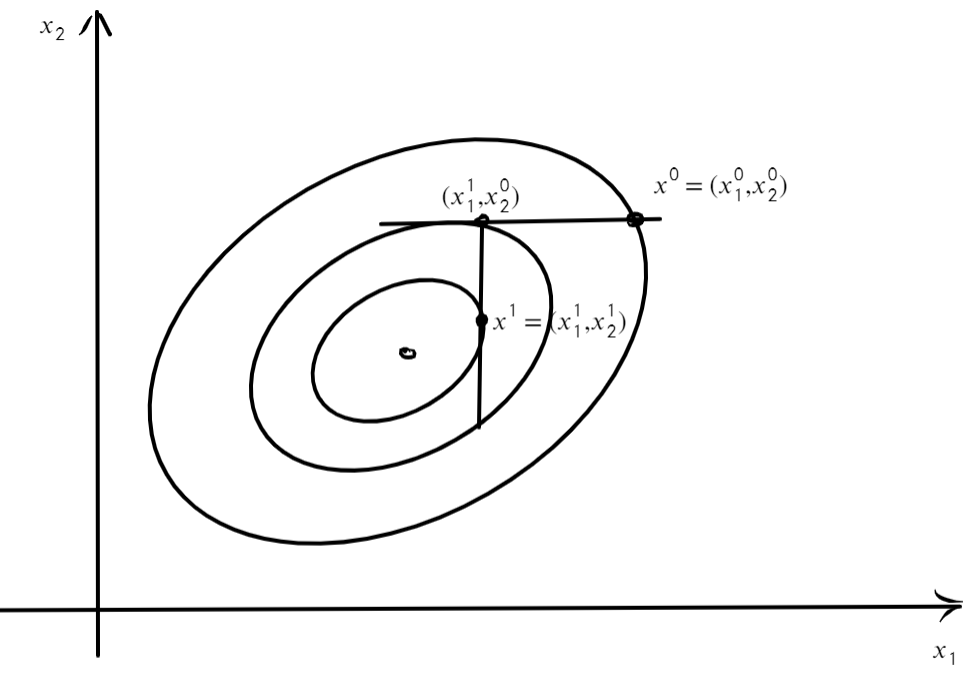
\includegraphics[scale=0.7]{img2.png}$$
	\subsection{Метод градиентного спуска.}
	Этот метод может быть применен для нахождения точки минимума любого функционала, для которого имеет смысл понятие градиента.\\\\
	$\bullet$ \textit{\textbf{Градиентом функции} $F(x_1,\ldots, x_n)$ называется вектор с координатами} $$\operatorname{grad}F(x)=\Big(\dfrac{\partial F}{\partial x_1}.\ldots, \dfrac{\partial F}{\partial x_n}\Big)^T.$$
	Пусть известно начальное приближение $x^0 = (x_1^0,\ldots, x_n^0).$ Из этой точки будем двигаться в направлении $-\operatorname{grad}F(x^0)$. Тогда путь, по которому мы будем перемещаться, имеет вид уравнения $$x = x^0 - t\operatorname{grad} F(x^0),\quad t\geq 0.$$
	Будем двигаться до тех пор, пока функция $F$ не достигнет своего минимума. Но для того, чтобы сформулировать это математически, нам нужно следить за изменением. Введем обозначение $$\varphi(t) = F(x^0 - t\operatorname{grad} F(x^0)).$$
	То есть мы останавливаемся в тот момент $t$, когда $$\varphi'(t) = \dfrac{d\varphi(t)}{dt} = 0.$$
	Выясним, какой вид имеет градиент в случае (2)
	$$\grad F(x) = 2(Ax - b).$$
	Учитывая, что $$\varphi(t) = (Ax, x) - 2(b,x),\quad x = x^0 - 2t(Ax^0 - b).$$
	Продифференцируем эту функцию по $t$:\begin{multline*}
		\dfrac{d}{dt}(Ax, x) = \Big(A\dfrac{dx}{dt}, x\Big) + \Big(Ax, \dfrac{dx}{dt}\Big) = 2\Big(\dfrac{dx}{dt}, Ax\Big) = 2(-\grad F(x^0), Ax) =\\= \ldots = 8t(Ax^0 - b) - 4(Ax^0 - b, Ax^0).
	\end{multline*}
	$$\dfrac{d}{dt} (b,x)= -2(Ax^0-b,b).$$
	Теперь вычислим
	$$\varphi'(t) = 8t(Ax^0 - b, A(Ax^0 - b)) - 4(Ax^0 - b, Ax^0 - b).$$
	А мы ищем $$\varphi'(t) = 0.$$
	То есть $$8t(Ax^0 - b, A(Ax^0 - b)) - 4(Ax^0 - b, Ax^0 - b) = 0$$
	и отсюда $$t = \dfrac{(Ax^0- b, Ax^0 - b)}{2(Ax^0 - b, A(Ax^0-b))}.$$
	Если мы нашли значение $t$, то мы можем уточнить вектор $x$:
	$$x^1 = x^0 - \dfrac{(Ax^0- b, Ax^0 - b)}{2(Ax^0 - b, A(Ax^0-b))}\cdot 2(Ax^0-b).$$
	Из $x^1$ точно так же переходим к $x^2$. Легко видеть, что эта формула не изменится, а она будет носить рекуррентный вид. Отсюда запишем \textbf{общий метод итерационного процесса градиентного спуска}. Для этого введем обозначение невязки $r = Ax - b$. Тогда $$x^{k+1} = x^k - \dfrac{(r^k, r^k)}{(Ar^k, r^k)}r^k,\quad r^k = Ax^k - b.\eqno(4)$$
	Геометрический смысл строится аналогично методу покоординатного спуска.
	$$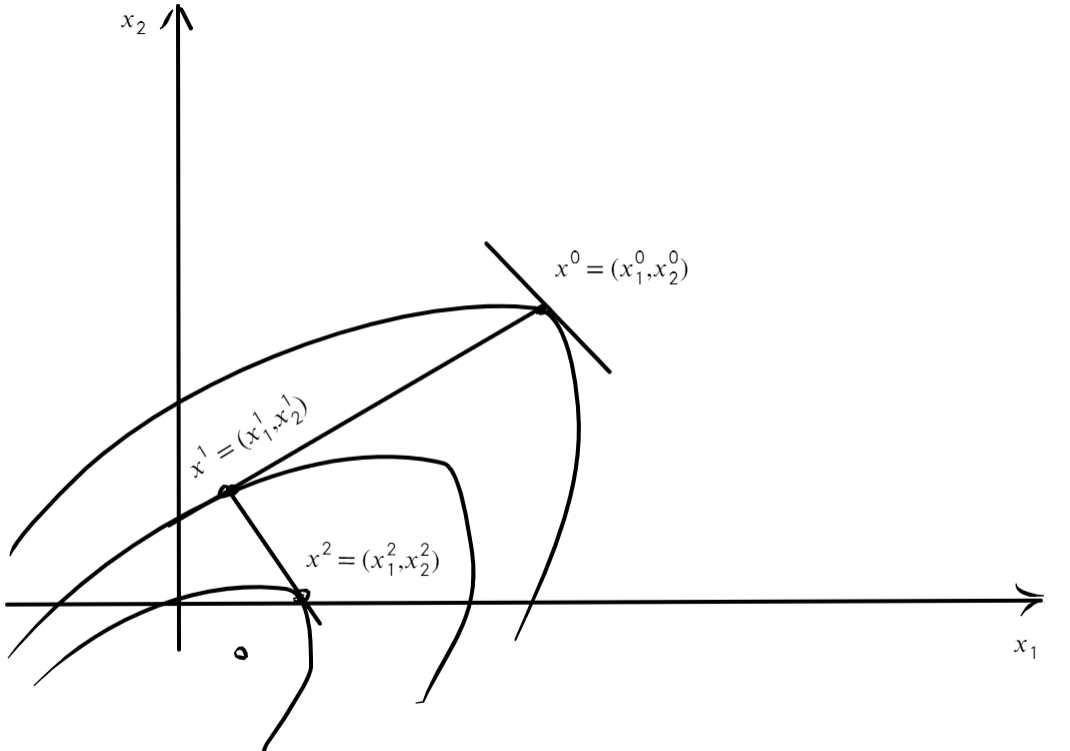
\includegraphics[scale = 0.7]{img3.png}$$
	Покажем сходимость метода.
	\begin{theorem}
		Если $A=A^T > 0$, то метод градиентного спуска $(4)$ сходится и для погрешности справедлива оценка $$\Norm{x^k - x^*} \leq \rho_0^k \Norm{x^0 - x^*},\quad \rho_0 = \dfrac{1 - \lambda_{min}(A)}{1 + \lambda_{max}(A)}.$$
	\end{theorem}
	\subsection{Метод релаксации.}
	Этот метод основан на минимизации функции ошибки $$z = x-x^*.$$
	Для того, чтобы работать с этой функцией, определим норму, порожденную матрицей $A$:
	$$\Norm{z}_A = \sqrt{(Az, z)}.$$
	Будем говорить, что итерационный процесс сходится в норме матрицы $A$, если $$\lim\limits_{k\to \infty}\Norm{z^k}_A = \lim\limits_{k\to\infty}\Norm{x^k-x^*} = 0.$$
	Предположим, что у нас имеется $s$-ое приближение к $x^*$ $$x^s = (x_1^s,\ldots, x_n^s).$$
	Под следующим приближением мы будем понимать такое значение вектора $x$, у которого меняется лишь $i$-ая компонента $$x^{s+1} = (x_1^s,\ldots, x_i^{s+1},\ldots, x_n^s).$$
	Формально можно записать итерационный процесс от $s$ итерации к $s+1$ как $$x^{s+1} = x^s - \alpha e_i,\quad \alpha = \operatorname{const},\ e_i = (0,\ldots, \underset{i}{1},\ldots, 0).$$
	Вычислим $$\Norm{z^{s+1}}_A^2 = (Az^{s+1}, z^{s+1})=\Big(A(z^s - \alpha e_i), z^s - \alpha e_i\Big)=\ldots = \Norm{z^s}_A^2 + \alpha ^2 a_{ii} - 2\alpha r_i^s.$$
	$$\Norm{z^{s+1}}_A^2 = \Norm{z^s}_A^2 + \dfrac{1}{a_{ii}}(\alpha a_{ii} - r_i^s)^2 - \dfrac{(r_i^s)^2}{a_{ii}}.\eqno(5)$$
	Как следует из формулы (5) минимум величины $z^{s+1}$ достигается при $\alpha = \dfrac{r_i^s}{a_{ii}}$.
	При этом $\alpha $ значение $r_i^{s+1} = 0$. Действительно, можно показать, что $$r_i^{s+1}=(Az^{s+1}, e_i)=(A(z^s - \alpha e_i),e_i) = (Az^s, e_i) - \alpha(Ae_i, e_i) = r_i^s - \alpha a_{ii} = 0$$
	при выбранном $\alpha = \dfrac{r_i^s}{a_{ii}}$.\\\\
	Однако при построении очередного приближения необязательно каждый раз минимизировать норму $$\Norm{z^{s+1}}_A^2.$$
	Нам достаточно потребовать, чтобы выполнялось
	$$\Norm{z^{s+1}}_A^2 < \Norm{z^{s}}_A^2.$$
	Оказывается, что последнее условие позволяет построить более оптимальные итерационные процессы. Если мы рассмотрим выполнение данного неравенства, то условие будет следующее $$|\alpha a_{ii} - r_i^s| < |r_i^s|.$$
	Теперь, если мы выберем $$\alpha = \omega \dfrac{r_i^s}{a_{ii}},\quad 0<\omega < 2,$$
	то получим следующее выражение
	$$r_i^{s+1} = (Az^{s+1}, e_i) = (1-\omega)r_i^s.$$
	Это соотношение позволяет записать общий метод --- \textbf{метод релаксации}, формулы которого имеют следующий вид:
	если предположить $$x^s = (x_1^{k+1},\ldots, x_{i-1}^{k+1}, x_i^k, x_{i+1}^k, \ldots, x_n^k)$$
	то 
	$$x^{s+1} = (x_1^{k+1},\ldots, x_{i-1}^{k+1}, x_i^{k+1}, x_{i+1}^k, \ldots, x_n^k).$$
	Тогда запишем
	$$x_i^{k+1} = (1-\omega)x_i^k - \omega \sum_{j=1}^{i-1} \dfrac{a_{ij}}{a_{ii}}x_j^{k+1} - \omega \sum_{j=i+1}^{n} \dfrac{a_{ij}}{a_{ii}} x_j^k + \omega \dfrac{b_i}{a_{ii}},\quad i = \overline{1,n},\ k=0,1,\ldots,\ 0 < \omega < 2.\eqno(6)$$
	Итерационный процесс (6) называется \textbf{методом релаксации}. Если $\omega \in (0,1)$, то получим \textbf{метод нижней релаксации}. Если $\omega \in (1,2)$, то это \textbf{метод верхней релаксации}. Если $\omega = 1$, то получим \textbf{метод полной релаксации}. Также при $\omega = 1$ мы получим метод Гаусса-Зейделя.\\\\
	Оптимальным значением $\omega$, которое дает максимальную скорость сходимости, является значение $\omega \in (1,2)$.
	\begin{theorem}
		Пусть $A = A^T > 0$, $0<\omega < 2$. Тогда метод релаксации сходится.
	\end{theorem}
	Запишем итерационный процесс (6) в матричной форме: если матрицу системы представить в виде суммы
	$$A = L + D + U$$
	тогда итерационный процесс (6) можно записать в матричном виде:
	$$(D + \omega L)\dfrac{x^{k+1} - x^k}{\omega} + Ax^k = b.$$
	Оптимальное значение $\omega$ часто определяется экспериментально.
	\subsection{Метод минимальных невязок.}
	Зададим начальное приближение $x^0$. Очередную итерацию, как в методе градиентного спуска, мы будем искать в виде $$x^1 = x^0 - \tau_1r^0.$$
	В некотором смысле функция невязки и есть величина градиента. По определению $$r^0 = Ax^0 - b.$$
	Причем $\tau_1$ мы выберем так, чтобы минимизировать функционал невязки $$(r^0, r^0) = \Norm{r^0}^2 \to \min.$$
	Докажем, что в качестве $\tau$ нам следует выбирать величину
	$$x^{k+1}= x^k - \tau _{k+1} r^k,\quad \tau_{k+1} = \dfrac{(Ar^k, r^k)}{(Ar^k, Ar^k)}\eqno(7)$$
	Формула (7) определяет \textbf{метод минимальных невязок}.
	\\\\
	Действительно так как $$r^{k+1} = r^k - \tau_{k+1} Ar^k,$$ то посчитаем норму невязки на $k+1$: $$\Norm{r^{k+1}}^2 = \Norm{r^k - \tau_{k+1} Ar^k}^2 = 
	\underbrace{(r^k, r^k)}_{=\Norm{r^k}^2} - 2\tau_{k+1} (Ar^k, r^k) + \tau^2(Ar^k, Ar^k).$$
	Отсюда видно, что $$\Norm{r^{k+1}}^2\to \min$$
	 при $$\tau_{k+1} = \dfrac{(Ar^k, r^k)}{(Ar^k, Ar^k)}.$$
	 \begin{theorem}
	 	Если $A = A^T>0$, то метод $(7)$ сходится и для погрешности метода справедлива оценка $$\Norm{A(x^k - x^*)}\leq \rho_0^k\Norm{A(x^0 - x^*)},\ k=0,1,\ldots\quad \rho_0 = \dfrac{1-\lambda_{\min}(A)}{1+\lambda_{\max}(A)}.$$
	 \end{theorem}
	 \chapter{Методы решения проблемы собственных значений (ПСЗ).}
	 \section{Общие положения ПСЗ.}
	 Сформулируем задачу, изучаемую в этой главе. Пусть матрица $A$ невырожденная, размерности $n\times n$ с элементами $a_{ij}$, $i,j=\overline{1,n}$. \\\\
	 $\bullet$ \textit{Число $\lambda$ называется \textbf{собственным значением} матрицы $A$, если} $$\exists x \ne 0 : Ax = \lambda x.\eqno (1)$$
	 \textit{Вектор $x$ называется \textbf{собственным вектором} матрицы $A$, соответствующим данному собственному значению матрицы $A$.}\\\\
	 Для существования задачи (1) необходимо, чтобы $$|A - \lambda E| = \begin{vmatrix}
	 a_{11} - \lambda & \ldots & a_{1n} \\
	 \vdots & \ddots & \vdots \\
	 a_{n1} & \ldots & a_{nn} - \lambda
	 \end{vmatrix} = 0\eqno (2)$$
	 $\bullet$ \textit{Левая часть равенства $(2)$ называется \textbf{характеристическим многочленом}. А само уравнение --- характеристическим (вековым) уравнением.}\\\\
	 Очевидно, что $|A-\lambda E|$ есть алгебраический многочлен степени $n$ от $\lambda$ со старшим коэффициентом $(-1)^n$
	 $$|A-\lambda E| = (-1)^n (\lambda^n - p_1\lambda ^{n+1} - \ldots - p_{n-1}\lambda - p_n) = (-1)^n P_n(\lambda)\eqno(3)$$
	 $\bullet$\textit{ Многочлен $P_n(\lambda)$ в формуле (3) называется \textbf{собственным многочленом} матрицы $A$.}\\\\
	 $\bullet$ \textit{Совокупность всех корней характеристического многочлена матрицы называется \textbf{спектром матрицы}.}
	 \\\\
	 Таким образом, задачу нахождения собственных значений и собственных векторов можно разбить на 3 этапа:\begin{itemize}
	 	\item построение собственного многочлена $P_n(\lambda)$ матрицы;
	 	\item решение уравнения $P_n(\lambda) = 0$ и нахождение его корней $\lambda_i(A)$; 
	 	\item отыскание нетривиальных решений систем вида $$Ax_i = \lambda_ix_i,\ i=\overline{1,n}.$$
	 \end{itemize}
	 Если необходимо знать все собственные значения и соответствующие векторы, то такая задача называется \textbf{полной ПСЗ}. Если необходимо знать одно или несколько собственных значений и соответствующих векторов, то такая задача называется \textbf{частиной ПСЗ}. На основе этого различают и методы решений задачи ПСЗ. Для решения полной ПСЗ используются прямые методы, а для частичной --- прямые и итерационные методы.\\\\
	 Рассмотрим вопрос об устойчивости ПСЗ. Исходными выходными данными в нашей задаче являются элементы матрицы $A$. Если мы имеем элементы матрицы $A$ с погрешностью, то вместо точного решения $x$ мы получим возмущенное решение, при этом этому $x$ будет соответствовать и возмущенное $\lambda$: $$(A + \delta A)(x + \delta x) = (\lambda + \delta \lambda)(x + \delta x).$$
	 Устойчивость задачи будет зависть от величины, называемой \textbf{коэффициентом перекоса матрицы}: $$\omega = \dfrac{\Norm{x}\cdot \Norm{y}}{|(x,y)|},$$
	 причем мы выбираем спектральную (третью) норму векторов. А $x$ и $y$ являются собственными векторами относительно матриц $A$ и $A^*$ соответственно: $$Ax = \lambda x,\quad A^* y = \overline{\lambda} y.$$
	 Если случай действительный, то $\lambda = \overline{\lambda}$, $A^* = A^T$. Очевидно, что $\omega \geq 1$. По определению фактически $$\omega = \dfrac{1}{|\cos \alpha|},$$ где $\alpha$ --- угол между векторами $x$ и $y$. Приведем основные оценки погрешности входных данных, которые обеспечивают устойчивость. В случае попарно различных собственных значений справедливы оценки $$|\delta \lambda_i| \leq \omega_i \Norm{\delta A}_\text{III}$$
	 $$\Norm{\delta x_i}\leq \Norm{x_i}\Big(\sum_{j=1}^n \dfrac{\omega _j}{|\lambda_i - \lambda_j|}\Big)\Norm{A}_\text{III},\ i\ne j\eqno(4)$$
	 Как следует из оценок (4), можно сделать следующие выводы:\begin{enumerate}
	 	\item собственное значение устойчиво относительно вариации матричных элементов, если соответствующий ему коэффициент перекоса мал; если коэффициент велик, то устойчивость будет плохой;
	 	\item собственный вектор устойчив относительно вариации, если все коэффициенты перекоса по всем собственным значениям достаточно малы;
	 	\item если матрица эрмитова, т.е. $A = A^*$, то все $\omega _i = 1$, а значит ПСЗ устойчива по всем $\lambda_i$, а проблема определения собственных векторов устойчива, если все $\lambda_i$ простые (отсутствуют кратные корни).
	 \end{enumerate}
	 \section{Метод Данилевского.}
	 Идея метода опирается на известный факт, что подобное преобразование матрицы $A$ не изменяет ее характеристического многочлена:
	 $$\exists S, |S| \ne0 : B=S^{-1}AS.$$
	 Действительно $$|B - \lambda E| = |S^{-1}AS - \lambda S^{-1}ES|=|S^{-1}|\cdot |A - \lambda E|\cdot |S| = |A-\lambda E|.$$
	 Для того, чтобы этот метод записать, рассмотрим каноническую форму Фробениуса:
	 $$\Phi = \begin{pmatrix}
	 	p_1 & p_2 & \ldots & p_{n-1} & p_n\\
	 	1 & 0 & \ldots & 0 & 0\\
	 	0 & 1 & \ldots & 0 & 0\\
	 	\vdots & \vdots & \ddots & \vdots & \vdots\\
	 	0 & 0 & \ldots & 1 & 0
	 \end{pmatrix}.$$
	 Непосредственная проверка показывает, что числа, стоящие в первой строке матрицы Фробениуса, являются коэффициентами собственного многочлена $P_n(\lambda)$. Действительно \begin{multline*}
	 	|\Phi - \lambda E| = \begin{vmatrix}
	 		p_1 - \lambda & p_2 & \ldots & p_{n-1} & p_n\\
	 		1 & - \lambda & \ldots& 0& 0\\
	 		\vdots & \vdots & \ddots & \vdots & \vdots\\
	 		0 & 0 & \ldots & 1 - \lambda & 0
	 	\end{vmatrix} = (p_1 - \lambda)(-\lambda)^{n-1} - \begin{vmatrix}
	 		p_2 & p_3 &\ldots& p_{n-1}& p_n\\
	 		1 & -\lambda & \ldots & 0 & 0\\
	 		0 & 1 & \ldots & 0& 0\\
	 		\vdots & \vdots & \ddots & \vdots & \vdots\\ 0& 0& \dots & 1-\lambda & 0
	 	\end{vmatrix} =\\= (p_1 - \lambda)(-\lambda)^{n-1} - p_2(-\lambda)^{n-2} - \ldots + (-1)^{n+1}p_n = (-1)^nP_n(\lambda).
	 \end{multline*}
	 \subsection{Построение собственного многочлена.}
	 Согласно методу Данилевского нам нужно найти такую матрицу $S$, что $$\Phi = S^{-1}AS.$$
	 Алгоритм метода Данилевского состоит в том, чтобы последовательными преобразованиями матрицы $A$ сделать ее вида Фробениуса. В зависимости от коэффициентов $a_{ij}$ различают два алгоритма\begin{enumerate}
	 	\item \textbf{Регулярный случай.}\\\\
	 	Нам нужно последнюю строку матрицы $A$ превратить в последнюю строку матрицы Фробениуса $$(a_{n1},\ldots, a_{nn-1},a_{nn})\to(0, \ldots, 1, 0).$$
	 	Предположим, что $a_{nn-1} \ne 0.$
	 	Разделим все элементы $n-1$-го столбца матрицы $A$ на элемент $a_{nn-1}$, вновь полученный $n-1$-ый столбец умножим на $a_{ni}$ и вычтем из столбцов номера $i$. Проделаем это для всех $i = 1,2,\ldots, n-2, n$, мы приведем последнюю строку матрицы $A$ к виду Фробениуса. Такое преобразование равносильно умножению матрицы $A$ справа на матрицу простой структуры $$M_{n-1} = \begin{pmatrix}
	 	1 & \ldots & 0 & 0\\
	 	\vdots & \ddots & \vdots & \vdots\\
	 	-\dfrac{a_{n1}}{a_{nn-1}} & \ldots & \dfrac{1}{a_{nn-1}} & -\dfrac{a_{nn}}{a_{nn-1}}\\
	 	0 & \ldots & 0 & 1
	 	\end{pmatrix}.$$
	 	После умножения получили $$B = AM_{n-1}.$$
	 	Домножим слева на $M^{-1}_{n-1}$ (она существует, так как $|M_{n-1}| = \dfrac{1}{a_{n-1}}\ne 0$) $$M^{-1}_{nn-1} = \begin{pmatrix}
	 	1 & \ldots & 0 & 0\\
	 	\vdots & \ddots & \vdots & \vdots\\
	 	a_{n1} & \ldots &a_{nn-1} & a_{nn}\\
	 	0 & \ldots & 0 & 1
	 	\end{pmatrix}.$$
	 	В итоге за счет двух умножений мы получили новую матрицу $$A_{1} = M_{n-1}^{-1}AM_{n-1} = \begin{pmatrix}
	 	a_{11}^1 & \ldots &a_{1n-1}^1& a_{1n}^1\\
	 	\vdots & \ddots & \vdots & \vdots \\
	 	a_{n-11}^1 &\ldots & a_{n-1n-1}^1 & a_{n-1n}^1\\
	 	0 & \ldots & 1 & 0
	 	\end{pmatrix}.$$
	 	Запишем, как пересчитываются элементы при умножении справа
	 	$$b_{ij} a_{ij} + a_{in-1} m_{n-1j},\quad j \ne n-1.$$
	 	$$b_{in-1} = a_{in-1}m_{n-1n-1},\quad i=\overline{1,n}$$
	 	Поменяется только $n-1$ строка матрицы, поэтому
	 	$$a_{ij}^1 = b_ij,\quad i = \overline{1,n-2}.$$
	 	$$a_{n-1j}^1 = \sum_{k=1}^{n}a_{nk}b_{kj},\quad j = \overline{1,n}.$$
	 	Далее нам нужно привести вторую строку в матрице $A_1$ к виду Фробениуса. То есть, нам нужно сделать единицу на месте $a_{n-1n-2}^1\ne 0$. Предположим, что он отличен от нуля. Теперь будем умножать на матрицу $M_{n-2}$ и $M_{n-2}^{-1}$. Эти матрицы формируются аналогично $M_{n-1}$, за исключением того, что отличной от единичной будет $n-2$-ая строка. После второго шага получим матрицу $$A_2 = M_{n-2}^{-1}A_1 M_{n-2}.$$
	 	И так далее. Будем предполагать, что все остальные элементы находящиеся на диагонали над главной диагональю отличны от нуля $$a_{nn-1}\ne 0, a_{n-1n-2}^1 \ne 0\ldots, a_{21}^{n-1}\ne 0.$$
	 	после выполнения $n-1$-го шага преобразования мы получим матрицу \begin{multline*}
	 		A_{n-1} = \underbrace{M_1^{-1}M_2^{-1}\ldots M_{n-1}^{-1}}_{S^{-1}}A\underbrace{ M_{n-1}\ldots M_2 M_1}_S = \begin{pmatrix}
	 			a_{11}^{n-1} & a_{12}^{n-1} & \ldots & a_{1n-1}^{n-1} & a_{1n}^{n-1} \\ 
	 			1 & 0 & \ldots & 0 & 0\\
	 			\vdots & \ddots & \vdots & \vdots \\
	 			0 & 0 & \vdots & 1& 0 
	 		\end{pmatrix} =\\= \begin{bmatrix}
	 			p_1 & p_2 & \ldots & p_{n-1}& p_n\\
	 			1 & 0 & \ldots & 0 & 0\\
	 			\dots & \ddots & \dots &\dots\\
	 			0 & 0 & \dots & 1 & 0
	 		\end{bmatrix} = \Phi.
	 	\end{multline*}
	 	По первой строке полученной матрицы составляется собственный многочлен матрицы $A$.
	 	\item \textbf{Нерегулярный случай}.\\\\
	 	Пусть процесс сведения матрицы $A$ к форме Фробениуса доведен до строки $k$ и при этом элемент $$a_{kk-1}^{n-k} = 0.$$ Дальнейше преобразование может быть выполнено по двум вариантам:\begin{enumerate}
	 		\item Мы должны проанализировать все элементы, стоящие левее элемента $a_{ki}^{n-k}\ne 0,\ i<k-1$. Столбец c номером $ki$ мы можем поменять местами с этим столбцом. Также необходимо поменять и строки с этими номерами. Далее по алгоритму регулярного случая;
	 		\item Все $a_{ki}^{n-k} = 0,\ i = \overline{1,k-1}$. В этом случае матрица
	 		$$A_{n-k} = \left(  \begin{tabular}{c|c}
	 			$\begin{tabular}{cc} 
	 			$\begin{matrix} a_{11}^{n-k}&\ldots & a_{1k-1}^{n-k}\\
	 			\vdots & \ddots & \vdots\\
	 			a_{k-11}^{n-k} & \ldots & a_{k-1k-1}^{n-k} \end{matrix}$ \end{tabular}$ & 
	 			$\begin{matrix} a_{1k}^{n-k} & \ldots & a_{1n}^{n-k}\\
	 			\vdots & \ddots & \vdots\\
	 			a_{k-1k}^{n-k} & \ldots & a_{k-1n}^{n-k} \end{matrix}$ \\ \hline 
	 			$\begin{matrix} 
	 			0 & \ldots & 0\\ 
	 			0 & \ldots & 0\\
	 			\vdots & \ddots & \vdots\\
	 			0 & \ldots & 0\end{matrix}$ & 
	 			$\begin{matrix} a_{kk}^{n-k} & \ldots & a_{kn}^{n-k}\\
	 			1 & \dots & 0\\
	 			\vdots & \ddots & \vdots\\
	 			0 & \dots & 0 \end{matrix}$ \end{tabular} \right) = \left(  \begin{tabular}{c|c}
	 			$\begin{tabular}{cc} $\begin{matrix} C_{n-k} \end{matrix}$ \end{tabular}$ & $\begin{matrix} D_{n-k} \end{matrix}$ \\ \hline $\begin{matrix} 0 \end{matrix}$ & $\begin{matrix} \Phi_{n-k} \end{matrix}$ \end{tabular} \right)$$
	 		Рассмотрим определитель, который является на данном этапе искомым $$|A_{n-k} - \lambda E| = \underbrace{|C_{n-k} - \lambda E_1|}_{P_{k-1}(\lambda)}\cdot \underbrace{| \Phi_{n-k} - \lambda E_2|}_{P_{n-k+1}(\lambda)} = 0.$$
	 		В этой формуле $E_1$ и  $E_2$ --- единичные матрицы порядка $(k-1)$ и $(n-k+1)$ соответственно. \\\\
	 		Поскольку второй сомножитель является определителем от матрицы Фробениуса, то для этого определителя мы можем выписать собственный многочлен по первой строке этой матрицы. Коэффициенты первого многочлена из этого произведения определяются по алгоритму регулярного случая. 
	 	\end{enumerate}
	 \end{enumerate}
	 \textbf{Замечания.}\begin{enumerate}
	 	\item Число операций в регулярном случае равно $O(n^3).$
	 	\item Чтобы повысить надежность вычислений, можно как в метода Гаусса с выбором элемента на каждом шаге преобразования матриц выбирать в качестве элемента, на который производится деление, можно ставить максимальный по модулю элемент матрицы, находящийся левее и выше него.
	 	\item Собственные значения найти по этому алгоритму мы не сможем, потому что мы лишь строим полином $P_n(\lambda) = 0.$
	 \end{enumerate} 
	 \subsection{Вычисление собственных векторов матриц.}
	 Собственный вектор является решением системы $$Ax = \lambda_i x,\quad i = \overline{1,n}.$$
	 Метод Данилевского позволяет построить систему собственных векторов матрицы $A$, используя вычисления, произведенные в процессе построения собственного многочлена. 
	 \begin{lem}
	 	Пусть имеются две матрицы $A$ и $B$, которые подобны между собой, то есть $B = S^{-1}AS$. Тогда если $y = (y_1,\ldots, y_n)^T$ является собственным вектором матрицы $B$, соответствующим собственному значению $\lambda$, то вектор $x = Sy$ есть собственный вектор матрицы $A$, соответствующий этому же значению $\lambda$.
	 \end{lem}\begin{Proof}
	 $$By = \lambda y \Rightarrow S^{-1}ASy = \lambda y\Rightarrow SS^{-1}A(Sy) = \lambda (Sy).$$
	 Значит $Sy$ --- есть собственный вектор матрицы $A$, соответствующий собственному значению $\lambda$.
	 \end{Proof}\\\\
	 Поскольку метод Данилевского приводит нас к матрице $\Phi = S^{-1}AS$, то можно воспользоваться леммой. Поскольку матрица $\Phi$ имеет простую структуру, то мы можем решать систему $$\Phi y = \lambda_i y.$$
	 Получится следующая система $$\begin{cases}
	 p_1y_1 + p_2y_2 + \ldots + p_ny_n = \lambda_iy_n,\\
	 y_1 = \lambda_i y_2,\\
	 \dotfill,\\
	 y_{n-1} = \lambda_iy_n.
	 \end{cases}$$
	 Здесь в качестве собственного вектора мы можем выбрать $$y = (\lambda_i^{n-1}, \lambda_i^{n-2}\ldots, \lambda_i,1),$$
	 если взять $y_n = 1$. Первое уравнение системы выполняется автоматически, поскольку $$p_1\lambda_i^{n-1} + p_2\lambda_i^{n-2} + \ldots + p_n = \lambda_i^n.$$
	 Для того, чтобы найти собственный вектор исходной матрицы $A$ нужно домножить на $S$:$$x = Sy =M_{n-1}\ldots M_1y.$$
	 При умножении вектора $y$ на $M_i$ будет изменяться только одна координата этого вектора. Такой способ построения собственных векторов годится только для регулярного случая.
	 \section{Метод Крылова.}
	 Метод Крылова основан на идее использования минимального многочлена матрицы аннулирующего заданный вектор.\\\\
	 $\bullet$ \textit{Многочлен $Q(\lambda) = \lambda^m + a_{m-1}\lambda^{m-1} + \ldots + a_m$ называется \textbf{аннулирующим} для матрицы $A$, если} $$Q(A) = A^m + a_1A^{m-1} + \ldots + a_mE = 0.$$
	 $\bullet$ \textit{Многочлен $Q(\lambda)$ называется \textbf{аннулирующим вектор} $c\ne 0$, если $$Q(A)c = 0.$$}
	 Если матрица $A$ имеет размерность $(n\times n)$, то $\exists m \leq n$, $m$ --- степень минимального многочлена.\\\\
	 $\bullet$ \textit{Аннулирующий многочлен наименьшей степени называется \textbf{минимальным многочленом} матрицы $A$.}\\\\
	 \textbf{\textit{Свойства:}}
	 \begin{enumerate}
	 	\item $\exists !$ минимальный аннулирующий многочлена матрицы $A$;
	 	\item $\exists !$ минимальный аннулирующий $c\ne 0$ многочлен матрицы $A$ и корни этого многочлена являются собственными значениями.
	 \end{enumerate}
	 \begin{theorem}
	 	[Гамильтона-Кели] Если $P_n(\lambda)$ --- собственный многочлен матрицы $A$, то $$P_n(A) = A^n - p_1A^{n-1} - \ldots - p_{n-1}A - p_nE = 0.$$ Следовательно, $P_n(\lambda)$ --- аннулирующий многочлен матрицы $A$.
	 \end{theorem}\subsection{Построение собственного многочлена.}
	 Рассмотрим произвольный ненулевой вектор $c^0$ (например, $(1,\ldots, 0)^T$), размерность которого согласована с матрицей $A$, и по этому вектору составим рекуррентную последовательность векторов:
	 $$c^0,\quad c^1=Ac^0,\quad c^2 = Ac^1 = A^2c^0,\ldots $$
	 Вычисление будем продолжать до тех пор, пока не получим вектор, являющийся линейной комбинацией предшествующих векторов. Мы дошли до какого-то шага, где $$c^m = q_1 c^{m-1} + q_2c^{m-2} + \ldots + q_mc^0,$$
	 при этом очевидно, что $c^0,\ldots, c^{m-1}$ линейно независимые, то есть $$\sum_{i=1}^{m}q_i^2 > 0.$$
	 Очевидно, что этот момент наступит по крайней мере в момент $m\leq n$.
	 Для определения коэффициентов $q_i$ запишем предельно возможную комбинацию, то есть в случае, когда $m=n$:
	 $$q_1c^{n-1} + q_2c^{n-2} + \ldots + q_nc^0 = c^n.$$
	 Распишем данную систему по координатам:
	 $$\begin{cases}
	 	q_1c_1^{n-1} + \ldots + q_nc_1^0 = c_1^n,\\
	 	\dotfill\\
	 	q_1c_n^{n-1} + \ldots + q_nc_n^0 = c_n^n.
	 \end{cases}\eqno(1)$$
	 (1) является неоднородной СЛАУ, определитель которой отличен от нуля лишь в случае линейной независимости векторов $c^0,\ldots, c^{n-1}$. Применим метод Гаусса для решения системы (1). При этом возможны два варианта:\begin{enumerate}
	 	\item Все $n$ шагов прямого хода метода Гаусса выполнимы $\Rightarrow$ система приводится к верхнему треугольному виду $$\begin{cases}
	 	q_1 + b_{12}q_2 + \ldots + b_{1n}q_n = g_1,\\
	 	q_2 + \ldots + b_{2n}q_{n} = g_2,\\
	 	\dotfill\\
	 	q_n = g_n
	 	\end{cases}\eqno(2)$$
	 	Тогда определитель системы (1) отличен от нуля и векторы $c^0,\ldots, c^{n-1}$ линейно независимые. Поэтому $q_1,\ldots, q_n$ найдутся единственным образом из системы (2) обратным ходом метода Гаусса. Нам осталось показать, что полученные коэффициенты $q_1,\ldots, q_n$ совпадают с соответствующими коэффициентами собственного многочлена $$P_n(\lambda)= \lambda^n - p_1\lambda^{n-1} - \ldots - p_n.$$ Для того, чтобы это доказать воспользуемся теоремой Гамильтона-Кели. Поскольку равенство $$P_n(A) = A^n - p_1A^{n-1} - \ldots - p_{n-1}A - p_nE = 0$$ справедливо для матрицы $A$, то умножим это равенство на $c^0$ справа и воспользуемся тем фактом, что по построению $$A^ic^0 = c^i,\ i =\overline{1,n}.$$
	 	В итоге получим $$p_1c^{n-1} + p_2c^{n-2} + \ldots + p_nc^0 = c^n.\eqno(3)$$
	 	С другой стороны, $$q_1c^{n-1} + q_2c^{n-2} + \ldots + q_nc^0 = c^n.\eqno(4)$$
	 	Вычитая из уравнения (3) уравнение (4), мы получим $$(p_1-q_1) c^{n-1} + (p_2-q_2)c^{n-2} + \ldots + (p_n-q_n)c^n = 0.$$
	 	Ввиду линейной независимости векторов $c^0, \ldots, c^{n-1}$ такое равенство возможно тогда, когда все коэффициенты в этом разложении обращаются в 0. Отсюда следует, что $$p_i = q_i,\ i = \overline{1,n}.$$
	 	Таким образом, мы построили собственный многочлен. 
	 	\item Прямой ход метода Гаусса возможен только на $m<n$ шагов преобразования. После их выполнения система будет иметь следующий вид:  
	 	$$\begin{cases}
	 	q_1 + b_{12}q_2 + \ldots + b_{1n}q_n = g_1,\\
	 	\dotfill\\
	 	q_m + \ldots + b_{mm}q_{n} = g_m,\\
	 	0 = 0.
	 \end{cases}\eqno(5)$$
		Следовательно, ранг системы (1) равен $m$ и среди всех векторов $c^0, \ldots, c^{n-1}$ есть только $m$ линейно независимых. Обозначим их $$c^0,\ldots, c^{m-1}.$$
		Поскольку эти векторы являются линейно независимыми и $m<n$, то мы можем записать соответствующую линейную комбинацию $$q_1c^{m-1} + q_2c^{m-2} + \ldots + c_mc^0 = c^m\eqno(6)$$
		Далее, записав эту систему покоординатно, и выбрав $m$ линейно независимых уравнений, мы найдем $q_1,\ldots, q_m$. Если домножить уравнение (6) на $c^0$ и воспользоваться тем, что $$A^ic^0 = c^i,\ i =\overline{1,n},$$ мы получим следующее уравнение $$\underbrace{(A^m - q_1A^{m-1} - \ldots - q_mE)}_{\varphi(A)}c^0 = 0.$$
		Мы таким образом получили, что $$\varphi(A)c^0 = 0,$$ то есть $\varphi(A)$ --- аннулирующий многочлен для вектора $c^0$. Тогда $$\varphi(\lambda) = \lambda^m - q_1\lambda^{m-1} - \ldots - q_m$$ и он является делителем любого другого многочлена матрицы $A$ аннулирующего вектор $c^0$. В частности, он является делителем и собственного многочлена $P(\lambda)$. Решая уравнение $$\varphi(\lambda) = 0,$$ мы найдем $\lambda_i$, $i=\overline{1,m}$, $m<n$ --- лишь часть спектра матрицы $A$. Следовательно, мы можем взять другое начальное приближение. И прийти либо к случаю 1, либо прийти к случаю 2, но получить другие коэффициенты.\\\\
		\textbf{Замечание}. Если изменением вектора $c^0$ не удается найти больше $m$ собственных чисел, то многочлен $\varphi(\lambda)$ будет являться минимальным многочленом матрицы $A$. Тогда получаются кратные значения.
	 \end{enumerate}
	 Для определения коэффициентов по методу Крылова требуется количество операций порядка $Q= O(n^3)$. Число операций умножения и деления $\dfrac{3}{2}n^2(n+1).$
	 \subsection{Вычисление собственных векторов матрицы.}
	 Рассмотрим для случая $m<n$. Пусть $\lambda_i$ --- корень минимального многочлена $\varphi(\lambda)$ матрицы $A$, аннулирующего вектор $c^0$. Собственный вектор $x_i$, соответствующий данному значению $\lambda_i$ будем находить в форме линейной комбинации построенных по методу Крылова собственных значений:
	 $$x_i = \beta_{i1} c^{m-1} + \beta_{i2}c^{m-2} + \ldots + \beta_{im}c^0.\eqno(7)$$
	 Подберем коэффициенты $\beta_{ij}$ таким образом, чтобы выполнялось равенство $$Ax_i = \lambda_ix_i\eqno(8).$$
	 Подставим сейчас уравнение (7) в уравнение (8) и воспользуемся соотношением $Ac^j = c^{j+1}$, $j = \overline{0,n-1}$. Тогда получим вместо (8) следующее равенство $$\beta_{i1}c^m + \beta_{i2}c^{m-1} + \ldots + \beta_{im} c^1 = \lambda_i\cdot (\beta_{i1} c^{m-1} + \beta_{i2}c^{m-2} + \ldots + \beta_{im}c^0).$$
	 Поскольку $c^m$ выражается через $c^0,\ldots,c^{m-1}$:
	 $$c^m = q_1c^{m-1} + \ldots + q_mc^0,$$ мы можем исключить его из полученного равенства. В итоге мы получим следующее уравнение $$(q_1\beta_{i1} + \beta_{i2} - \lambda_i\beta_{i1})c^{m-1} + (q_2\beta_{i1} + \beta_{i3} - \lambda_i\beta_{i2})c^{m-2}) + \ldots + (iq_m\beta_{i1}-\lambda_i\beta_{im})c^0 = 0$$
	 Так как векторы $c^0,\ldots, c^{m-1}$ по построению линейно независимые, то нам нужно, чтобы все коэффициенты в этой сумме одновременно обращались в ноль.
	 $$ \begin{cases}
	 	q_1\beta_{i1} + \beta_{i2} - \lambda_i\beta_{i1} = 0,\\
	 	\dotfill\\
	 	q_{m-1}\beta_{i1} + \beta_{im} - \lambda_i\beta_{im-1} = 0\\
	 	q_m\beta_{i1} - \lambda_i\beta_{im} =0
	 \end{cases}\eqno(9)
	 $$
	 Легко видеть, что эту систему можно разрешить и последовательно находить $\beta_{ik}$ через $\beta_{i1}$:
	 $$
	 \begin{cases}
	 	\beta_{i2} = (\lambda_i - q_1)\beta_{i1},\\
	 	\beta_{i3} = (\lambda_i^2 - q_1\lambda_i - q_2)\beta_{i1},\\
	 	\dotfill\\
	 	\beta_{im} = (\lambda_i^{m-1} - q_1\lambda_i^{m-2}-\ldots - q_{m-1})\beta_{i1},\\
	 	(\lambda_i^m - q_1\lambda_i^{m-1} - \ldots - q_m)\beta_{i1} = 0
	 \end{cases}$$
	 Последнее равенство выполнено, потому что $\lambda_i$ --- собственные значения. Следовательно, мы можем построить вектор $x$. Обычно полагают 
	 $$\begin{cases}
	 	\beta_{i1} = 1,\\
	 	\beta_{i2} = \lambda_i - q_1,\\
	 	\beta_{i3} = \lambda_i^2 - q_1\lambda_i - q_2,\\
	 	\dotfill\\
	 	\beta_{im} = \lambda_i^{m-1} - q_1\lambda_i^{m-2} - \ldots - q_{m-1}.
	 \end{cases}\eqno(10)$$
	И по формуле (7) строим собственный вектор. Описанный способ нахождения собственных вектор справедлив независимо от случая $m=n$ или $m< n$.
	Если данному собственному значению принадлежат несколько собственных векторов, то для их отыскания необходимо выбрать другие начальные векторы $c^0$ и повторить указанную процедуру.
	\section{Итерационный метод вращений решения ППСЗ.}
	Рассмотрим для простоты случай, когда матрица $A$ действительная и симметричная, т.е. $A = A^T$, $a_{ij} \in \Rm$.
	\subsection{Предварительные сведения.}
	Известно, что всякая симметричная действительная матрица может быть приведена к диагональному виду подобным преобразованием. Иными словами, имеет место разложение вида $$A = U \Lambda U^{-1},\eqno(1)$$
	где $U$ --- это ортогональная матрица, $\Lambda$ --- диагональная матрица, причем диагональными элементами в этой матрице являются собственные значения $\lambda_i$, $i = \overline{1,n}$ матрицы $A$. 
	При этом столбцы матрицы $U$ являются столбцами координат собственных векторов, соответствующих этим собственным значениям. \\\\
	$\bullet$ \textit{Это разложение называется \textbf{каноническим}, или \textbf{спектральным} разложением матрицы $A$.}\\\\
	Поскольку $U^T = U^{-1}$, мы можем записать наряду с (1) $$U^T AU = \Lambda\eqno(2).$$
	Таким образом, можно построить последовательных ортогональных (подобных) преобразований, позволяющих неограниченно уменьшать модули недиагональных элементов матрицы $A$. Меру близости $A$ к диагональному виду определим следующим образом. Введем функцию $$\sigma_i(A) = \sum_{j=1, i\ne j}^{n}|a_{ij}|^2,\ i=\overline{1,n}\eqno(3)$$
	Теперь за меру близости матрицы $A$ к диагональной мы примем число $$t(A) = \sigma_1 + \ldots + \sigma_n = \sum_{i,j, i \ne j}^{}|a_{ij}|^2.\eqno(4)$$
	Эта функция и будет являться критерием близости матрицы $A$ к диагональной. Понятно, что $t(A)$ должно стремиться к нулю.  \\\\
	Пусть с помощью преобразования подобия с ортогональными матрицами построена последовательность $$A=A^0, A^1,\ldots, A^k.$$
	$\bullet$ \textit{Процесс называется \textbf{монотонным}, если $t(A^k) < t(A^{k-1})$}.
	\subsection{Алгоритм метода.}
	По заданной матрице $A$ будем строить последовательность матриц $A^k$ так, что каждая следующая матрица $A^{k+1}$ получается из матрицы $A^k$ при помощи преобразования подобия с матрицей вращения $T_{ij}$ (п. 2.7.3). Предположим, что преобразования доведенные до шага $k$ и построена матрица $A^k = \{a_{ij}^k\}$. Найдем в ней наибольший по модулю недиагональный элемент $a_{ij}^k, i\ne j$. Поскольку матрица $A$ симметрическая, то искать элемент можно в верхнем треугольнике $i < j$ (если таких элементов несколько, то можно взять любой из них в качестве максимального по модулю элемента). По индексам $i$, $j$ строим матрицу $T_{ij}^k = T_{ij}(\varphi^k)$. Значение угла $\varphi$ мы определим ниже. Образуем матрицу $$A^{k+1} = (T_{ij}^k)^TA^kT_{ij}^k.\eqno(5)$$
	Такое преобразование является подобным. У этих матриц будет совпадать характеристический многочлен. Для вычисления введем матрицу $$B^k = A^kT_{ij}^k.$$
	У матрицы $B$ от $A^k$ будут отличаться только столбцы под номерами $i$ и $j$, а именно
	$$\begin{cases}
		b^k_{li} = a_{li}^k\cos \varphi^k + a_{lj}^k\sin \varphi^k,\\
		b^k_{lj} = -a_{li}^k\sin\varphi^k + a_{lj}\cos\varphi^k.
	\end{cases},\quad l = \overline{1,n}\eqno(6)$$
	Если мы будем умножать матрицу $B^k$ слева на $(T_{ij}^k)^k$, то в матрице $$A^{k+1} = (T_{ij}^k)^kB$$ будут отличаться две строки по сравнению с матрицей $B^k$, а именно $i$-ая и $j$-ая строки
	$$\begin{cases}
		a_{il}^{k+1} = b_{il}^k \cos\varphi^k + b_{jl}^k\sin\varphi^k,\\
		a_{jl}^{k+1} = -b_{il}^k \sin\varphi^k + b_{jl}^k\cos\varphi^k.
	\end{cases},\quad l = \overline{1,n}\eqno(7)$$
	На основании формул (6) и (7) мы сразу можем записать выражение элементов матрицы $A^{k+1}$ через элементы матрицы $A^k$:
	\begin{multline*}
		a_{ij}^{k+1} = b_{ij}^k\cos\varphi^k + b_{jj}^k\sin\varphi^k = (-a_{ii}^k\sin\varphi^k + a_{ij}^k\cos\varphi^k)\cos\varphi^k + (-a_{ji}^k \sin\varphi^k + a_{jj}^k\cos\varphi^k)\sin\varphi^k
	\end{multline*}
	Учитывая симметрию задачи, мы упростим и получим $a_{ij}^k = a_{ji}^k$. В итоге $$a_{ij}^{k+1} = a_{ij}^k \cos 2\varphi^k + \dfrac{1}{2}(a_{jj}^k - a_{ii}^k)\sin 2\varphi^k.\eqno(8)$$
	Выберем теперь угол $\varphi^k$ так, чтобы элемент $a_{ij}^{k+1}$ обратился в нуль. Требование того, что $a_{ij}^{k+1} = 0$ приводит к формулам $$\tg2\varphi^k = \dfrac{2a_{ij}^k}{a_{ii}^k - a_{jj}^k},\quad |\varphi^k|\leq \dfrac{\pi}{4}\eqno(9)$$
	$$\cos2\varphi^k = \dfrac{1}{\sqrt{1+\tg^22\varphi^k}}.$$
	Пользуясь последней формулой, вычислим $$\cos\varphi^k = \sqrt{\dfrac{1+\cos2\varphi^k}{2}}\eqno(10)$$
	Аналогично
	$$\sin\varphi^k = \pm \sqrt{\dfrac{1 - \cos2\varphi^k}{2}}\eqno (10)$$
	Чтобы выполнялось условие $|\varphi|\leq \pi/4$, знак в формуле для $\sin$ знак выбирается тот же, что и у выражения $$a_{ij}^k (a_{ii}^k - a_{jj}^k)\eqno(11)$$
	Сформулируем алгоритм рассматриваемого метода. Для определения матриц $\Lambda$ и $U$ в разложении (1) по формуле (5) строим последовательность матриц $$A^0 = A,\ A^1,\ A^2,\ \ldots,\ A^k,\ldots \longrightarrow \Lambda$$
	При этом для вычисления матриц на каждом шаге метода используются формулы (9), (10), (11), (6) и (7). Одновременно с построением последовательности матриц $A^k$ строим последовательность матриц $U$:
	$$U^0 = E,\ U^1,\ U^2,\ \ldots,\ U^k,\ \ldots\longrightarrow U$$
	где каждое $$U^{k+1} = U^k \cdot T_{ij}^k,\quad k=0,1,\ldots$$
	Вычисления продолжаем до тех пор, пока не выполнится условие $$|t(A^{k+1})| \leq \epsilon,$$
	где $t(A)$ --- мера близости, определяемая по формуле (4). В итоге в рамках заданной точности $\epsilon$ диагональные элементы последней матрицы $A^{k+1}$ принимаются за искомые собственные значения $$\lambda_i = a_{ii}^{k+1},\quad i=\overline{1,n}$$
	Столбцы матрицы $U^{k+1}$ принимаются за координаты собственных векторов, соответствующих этим собственным значениям.
	\subsection{Сходимость итерационного процесса.}
	Если мы докажем, что $t(A^k) \xrightarrow[k\to \infty]{}0$, то мы получим сходящийся итерационный процесс. Рассмотрим величину $$t(A^{k+1}) = \sum_{l=1}^{n}\sum_{m=1, m\ne l}^{n}(a_{lm}^{k+1})^2$$
	Как следует из формул (6) и (7) при подобном преобразовании вращения сумма недиагональных 
	элементов всех строк матрицы $A^{k+1}$ кроме $i$-ой и $j$-ой остается неизменной. То есть изменение $t(A^{k+1})$ от $t(A^k)$ зависит только от $i$-ой и $j$-ой строки. Докажем это. С одной стороны, $$(b_{li}^k)^2 + (b_{lj}^k)^2 = (a_{li}^k)^2 + (a_{lj}^k)^2.$$
	Теперь мы возьмем $i$-ую и $j$-ую строки, и для них выполняется следующее соотношение:
	$$(a_{ij}^{k+1})^2 + (a_{jl}^{k+1})^2 = (b_{il}^k)^2 + (b_{jl}^k)^2.$$
	Для всех $l\ne i, l \ne j$ $$b_{il} = a_{il},\quad b_{jl} = a_{jl}$$ по построению.
	Следовательно, $$(a_{ij}^{k+1})^2 + (a_{jl}^{k+1})^2 = (a_{il}^k)^2 + (a_{ij}^k)^2,\quad l \ne i, l\ne j.$$
	При $l = i$ и $l= j$ у нас будут два равенства $$(a_{ii}^{k+1})^2 + (a_{ji}^{k+1})^2 = (a_{ii}^k)^2 + (a_{ji}^k)^2,$$
	$$(a_{ij}^{k+1})^2 + (a_{jj}^{k+1})^2 = (a_{ij}^k)^2 + (a_{jj}^k)^2.$$
	Теперь мы учтем тот факт, что при построении $A^{k+1}$ мы выбирали угол $\varphi$ таким образом, что $a_{ij}^{k+1} = a_{ji}^{k+1}$. В итоге из этих двух равенств у нас получится 
	$$(a_{ii}^{k+1})^2 + (a_{jj}^{k+1})^2 = (a_{ii}^{k})^2 + (a_{jj}^{k})^2 + 2(a_{ij}^k)^2.$$
	Из этого равенства следует, что изменение от итерации к итерации определяется величиной $2(a_{ij}^k)^2$. Тогда мы можем записать следующее соотношение $$t(A^{k+1}) = \sum_{l=1}^{n}\sum_{m=1, m\ne l}^{n}(a_{lm}^{k+1})^2 = \sum_{l=1}^{n}\sum_{m=1, m\ne l}^{n} (a_{lm}^k)^2 - 2(a_{ij}^k)^2.$$
	Это равенстве есть ничто иное как $$t(A^{k+1}) = t(A^k) - 2(a_{ij}^k)^2\eqno(12)$$
	Так как $a_{ij}^k$ есть наибольший по модулю недиагональный элемент, он отличен от нуля. Тогда $$t(A^{k+1}) < t(A^k).$$
	Таким образом, мы доказали сходимость итерационного процесса. Теперь покажем скорость стремления к нулю: $$t(A^k)\leq n(n-1)(a_{ij}^k)^2.$$
	Отсюда $$(a_{ij}^k)^2\geq\dfrac{1}{n(n-1)}t(A^k).$$
	Используем формулу (12) $$t(A^{k+1})\leq t(A^k) - \dfrac{2}{n(n-1)}t(A^k) = qt(A^k),\quad q = 1-\dfrac{2}{n(n-1)}.$$
	В случае, если $n\geq 2$, то $0\leq q \leq 1$. Используя последнее неравенство, можно записать $$t(A^k)\leq qt(A^{k-1})\leq \ldots \leq q^kt(A^0).$$
	Учитывая то, что $A^0 = A$, окончательно получим оценку $$t(A^k)\leq q t(A)\eqno(13)$$
	Из (13) следует, что $t(A^k)\xrightarrow[k\to \infty]{}0$, то есть процесс этот сходящийся и скорость сходимости равна скорости сходимости геометрической прогрессии со знаменателем $q<1$. \\\\
	\textbf{Замечания.}\begin{enumerate}
		\item Необходимо выполнить $\dfrac{n(n-1)}{2}\sim O(n^2)$ сравнений. Можно уменьшить объем вычислений, если взять наибольшую из сумм (3) $\sigma_i(A^k)$. В качестве $a_{ij}^k$ можно брать максимальный элемент в этой строке, относящейся к $\sigma_i$. В этом случае нам понадобится $O(n)$ сравнений. При этом на следующей итерации меняются только величины $$\sigma_i(A^{k+1})=\sigma_i(A^k) + (a_{ii}^{k+1})^2 - (a_{ii}^k)^2 - (a_{ij}^k)^2$$ и $\sigma_j(A^{k+1}) = \sigma_j(A^k) +\sigma_i(A^k) - \sigma_i(A^{k+1}).$
		\item Из формулы (13) можно получить априорную оценку количества итераций. Для того, чтобы получить точность $\epsilon$ нужно совершить $k$ итераций, где $$k \geq \dfrac{\lg\epsilon - \lg t(A)}{\lg q}$$
		\item Предельное количество арифметических операций требуемых для выполнения одного шага алгоритма $Q(n) = 2n^2 + O(n)$, $n\to\infty$.
	\end{enumerate}
	\section{Степенной метод.}
	Данный метод применяется для решения частной ПСЗ.
	\subsection{Нахождение наибольшего по модулю собственного значения и соответствующего собственного вектора.}
	Пусть матрица $A$ вещественная и обладает полной системой $n$ линейно независимых собственных векторов. Это обеспечивается в тех случаях, когда собственные значения различны между собой или матрица $A$ симметрическая.\\\\
	Обозначим собственные значения и собственные векторы $\lambda_1$, $\ldots$, $\lambda_n$ и соответствующие им собственные векторы $x^1$, $\ldots$, $x^n$. Пусть $\lambda_i$ перенумерованы в порядке невозрастания модулей, то есть $$|\lambda_1| > |\lambda_2| \geq |\lambda_3| \geq \ldots \geq |\lambda_n|.$$
	Перед нами стоит задача нахождения наибольшего по модулю собственного значения и соответствующего ему собственного вектора.\\\\
	Возьмем произвольный вектор $y^0 = (y_1^0,\ldots, y_n^0)^T$ и построим рекуррентную последовательность:
	$$y^0,\quad y^1 = Ay^0,\quad y^2 = Ay^1 = A^2y^0,\quad\ldots,\quad y^k = Ay^{k-1}=\ldots=A^ky^0,\ldots$$
	Разложим $y^0$ по системе полных векторов: $$y^0 = \alpha_1 x^1 + \ldots + \alpha_nx^n. \eqno(1)$$		
	Выразим $y^k$ по координатам, учитывая, что $A^k x^i = \lambda_i^k x^i$:
	$$y^k_s =\beta_{1s}\lambda_1^k + \beta_{2s}\lambda^k_2 + \ldots + \beta_{ns}\lambda_n^k ,\quad s=\overline{1,n},\beta_{is} = \alpha_i x^i_s, i =\overline{1,n}.\eqno(2)$$
	Рассмотрим отношение компонент итерационной последовательности на $k$-ом и $k+1$-ом шаге. То есть запишем отношение \begin{multline*}
		\dfrac{y_s^{k+1}}{y_s^k} = \dfrac{\beta_{1s}\lambda_1^{k+1} + \beta_{2s}\lambda^{k+1}_2 + \ldots + \beta_{ns}\lambda_n^{k+1}}{\beta_{1s}\lambda_1^k + \beta_{2s}\lambda^k_2 + \ldots + \beta_{ns}\lambda_n^k} = \lambda_1\cdot \dfrac{1 + \gamma_{2s} \mu_2^{k+1} + \ldots + \gamma_{ns}\mu_n^{k+1}}{1 + \gamma_{2s} \mu_2^{k} + \ldots + \gamma_{ns}\mu_n^{k}};\\ \gamma_{is} = \dfrac{\beta_{is}}{\beta_{1s}}, \mu_i = \dfrac{\lambda_i}{\lambda_1}, i =\overline{2,n}.\qquad(4)
 	\end{multline*}
	Очевидно, что $|\mu_i| <1$. Тогда при $k\to\infty$ получится, что $$\dfrac{y_s^{k+1}}{y_s^k} = \lambda_1 + O(|\mu_2|^k).$$
	Отсюда следует, что в качестве $\lambda_1$ при достаточно больших $k$ в пределах принятой точности можно взять величину $$\lambda_1 \approx \dfrac{y_s^{k+1}}{y_s^k}.\eqno(5)$$
	Правая часть в формуле (5) зависит от $s$. Если будет одинаковое значение при всех $s$ в пределах принятой точности, то это является некоторой гарантией достигнутой точности при достаточно больших $k$.\\\\
	Теперь найдем соответствующий собственный вектор. Для этого используем формулу (2), учитывая тот факт, что при достаточно больших $k$ все слагаемые начиная со второго можно отбросить. В итоге при $k\to\infty$ сохранится лишь первое слагаемое. А отсюда мы можем записать, что 
	$$x^1\approx \dfrac{1}{\alpha_1 \lambda_1^k}y^k.$$
	Понятно, что $\alpha_1$ --- это константа, которую мы заранее не знаем. Но учитывая тот факт, что собственный вектор находится с точностью до константы, то мы можем это заменить как $$x^1\approx \dfrac{1}{\alpha_1 \lambda_1^k}y^k = c_k^yk,\eqno(6)$$ где $c_k$ --- произвольная константа. Обычно берут $c_k = 1$.\\\\
	Видно, что скорость убывания величины $O(|\mu_2|^k)$ равна скорости убывания геометрической прогрессии с показателем меньше 1. Можно попытаться увеличить скорость сходимости, а значит уменьшить количество итераций для достижения необходимой точности. В случае, если матрица $A = A^T$ можно увеличить скорость сходимости итерационного процесса. Поскольку для симметрической матрицы систему собственных векторов всегда модно считать ортонормированной. Это означает $$(x_i, x_j) = \delta_{ij}, \quad i,j = \overline{1,n},$$ $\delta_{ij}$ --- символ Кронекера. Используя формулу (3), можно вычислить скалярное произведение $$(y^k, y^k) = \alpha_1^2\lambda_1^{2k} + \alpha_2^2 \lambda_2^{2k} + \ldots + \alpha_n^2 \lambda_n^{2k}.$$
	Наряду с этим скалярным произведением рассмотрим $$(y^{k+1}, y^k) =  \alpha_1^2\lambda_1^{2k+1} + \alpha_2^2 \lambda_2^{2k+1} + \ldots + \alpha_n^2 \lambda_n^{2k+1}.$$
	Легко видеть, что если мы составим отношение этих скалярных произведений, то есть вместо отношения компонент векторов рассмотрим отношение $$\dfrac{(y^{k+1}, y^k)}{(y^k, y^k)} = \lambda_1 + O(|\mu_2|^{2k})$$ при выделении главной части. То есть на порядок увеличилась скорость. Но мы платим операциями вычисления скалярного произведения. Отсюда в качестве $\lambda_1$ можно взять $$\lambda_1 \approx \dfrac{(y^{k+1}, y^k)}{(y^k, y^k)}\eqno(7).$$ В данном случае в качестве собственного вектора будет значение $y_k$.\\\\
	\textbf{Замечания.}\begin{enumerate}
		\item Понятно, что если мы будем каждый раз считать $y^k$, то нам надо умножать на матрицу $A$, то есть компоненты этого вектора будут либо возрастать, если $|\lambda_1| > 1$, либо неограниченно убывать, когда $|\lambda_1| < 1$. За счет этого получаются векторы с очень большими по модулю компонентами. Чтобы избежать чрезмерного роста в абсолютной величине координат векторов $y^k$ (либо чрезмерного убывания), целесообразно эти векторы нормировать. При этом вместо последовательности $$y^0,\quad y^1 = Ay^0,\quad\ldots,\quad y^k = A^ky^0$$ мы будем строить последовательность $$z^0 = y^0,\quad z^1 = \alpha_1 Ay^0,\quad z^2\alpha_2A^2y^0,\quad\ldots,\quad z^k = \alpha_kA^ky^0.$$
		Здесь $\alpha$ --- это нормирующий множитель. Например, можно взять$$\alpha_k = \dfrac{1}{\Norm{A^ky^0}}.$$ Если выбрать первую норму, то у нас получится одна компонента единица, а остальные меньше единицы. Для получения приближения к собственному значению $\lambda_1^k$, $k=1,2,\ldots$ в случае нормировки надо брать отношение координат $Az^k$ и $z^k$.
		\item В качестве критерия останова итерационного процесса используется условие $$|\lambda_1^{k+1} - \lambda_1^k|\leq \epsilon.$$
	\end{enumerate}
	\subsection{Нахождение наименьшего по модулю собственного значения (метод обратных итераций).}
	Будем предполагать, что по-прежнему 
		$$|\lambda_1| \geq |\lambda_2| \geq |\lambda_3| \geq \ldots > |\lambda_n|.$$ Обозначим через $\nu_i, i = \overline{1,n}$ собственные значения матрицы $A^{-1}$. Далее, зная соотношения между матрицей и обратной к ней, получаем $$\nu_i = \dfrac{1}{\lambda_i},\quad \nu_{\max} = \nu_n = \dfrac{1}{\lambda_{\min}} = \dfrac{1}{\lambda_n}.$$
	Поэтому для того, чтобы найти минимальное по модулю собственное число матрицы $A$, достаточно найти максимальное по модулю собственное число матрицы $A^{-1}$. После этого нужно применить алгоритм, описанный в пункте 5.1. \\\\
	Можно организовать вычисления так, чтобы не нужно было обращать матрицу $A$. Для этого надо каждое $y^k$ приближение находить из системы $$Ay^k = y^{k-1},\quad k=1,2,\ldots.$$
	Легко видеть, что построенная таким образом итерационная последовательность будет сходитсья со скоростью геометрической прогресси со знаменателем $$\Big|\dfrac{\nu_{n-1}}{\nu_n}\Big| = \Big|\dfrac{\lambda{n}}{\lambda_{n-1}}\Big|$$
	Аналогичным способом вычисляется собственный вектор, т.е. он будет равен $y^k$.\\\\
	Если на первой итерации построить $LU$ разложение матрицы $A$, то все последовательные операции могут быть реализованы за $O(n^2)$ арифметических операций. Аналогично, если $A = A^T$, то можно повысить скорость сходимости также как и в пункте 5.1. То есть вместо отношения $\dfrac{y^{k+1}}{y^k}$ будем рассматривать $\dfrac{(y^{k+1}, y^k)}{(y^k, y^k)}$, при этом скорость сходимости будет на порядок больше: $O\Big(\big|\dfrac{\nu_{n-1}}{\nu_n}\big|^{2k}\Big).$
	\subsection{Случай кратного доминирующего собственного значения.}
	Известно, что есть кратный корень. Причем он является максимальным по модулю по отношению к остальным собственным значениям, то есть $$\lambda_1 = \lambda_2 = \ldots = \lambda_r$$ и $$|\lambda_1| > |\lambda_{r+1}|\geq \ldots \geq |\lambda_n|.$$
	В данном случае разложение (2) примет следующий вид $$y^k = \lambda_1^k (\alpha_1 x^1 + \ldots + \alpha_rx^r) + \alpha_{r+1}\lambda_{r+1}^k x^{r+1} + \ldots + \alpha_n\lambda^k_nx^n.$$
	Легко видеть, что $$y_s^k = \beta_{1s}\lambda_1^k + \beta_{r+1s}\lambda_{r+1}^k + \ldots + \beta_{ns}\lambda_n^k,\quad \beta_{1s} = \alpha_1x_s^1 + \ldots + \alpha_rx_s^r, \beta_{is} = \alpha_sx_s^i, i = \overline{r+1, n}.$$
	Так же как и в случае (5.1) мы получим $$\dfrac{y_s^{k+1}}{y_s^k} = \lambda_1 + O(|\mu_{r+1}|^k),\quad \mu_{r+1} = \dfrac{\lambda_{r+1}}{\lambda_1}.$$
	Эта формула практически приводит к формуле (5): $$\lambda_1 \approx \dfrac{y_s^{k+1}}{y_s^k}.$$
	Но для найденного значения $\lambda$ мы получим собственный вектор, совпадающий с $y^k$. Но в данном случае $$y^k = \lambda_1^k (\alpha_1x^1 + \ldots + \alpha_rx^r).$$ Для того, чтобы найти полную систему векторов, нам нужно изменить $y^0$ и получить другую итерационную последовательность, которая в принципе даст нам то же самое $\lambda$, но значения будут другие. Они и обеспечат нам получения новых собственных векторов. И так далее $r-2$ раз.
	\subsection{Случай двух наибольших собственных значений, отличающихся знаками.}
	Пусть $\lambda_2 = -\lambda_1$. Тогда мы будем рассматривать последовательность $$|\lambda_1| > |\lambda_3| \geq \ldots \geq |\lambda_n|.$$
	Тогда здесь $$y^k = \lambda_1^k ( \alpha_1x^1 + (-1)^k\alpha_2x^2) + \alpha_3x^3 + \ldots + \alpha_n x^n.$$
	Учитывая, что знак в скобке будет все время меняться в зависимости от $k$, то рассмотрим четные и нечетные итерации:
	$$y^{2k} = \lambda_1^{2k} ( \alpha_1x^1 + \alpha_2x^2) + \alpha_3x^3 + \ldots + \alpha_n x^n,$$
	$$y^{2k+1} = \lambda_1^{2k+1} ( \alpha_1x^1 - \alpha_2x^2) + \alpha_3x^3 + \ldots + \alpha_n x^n.$$
	Если коэффициенты $\alpha_1\ne \alpha_2$, то тогда можем рассматривать отношение четных и нечетных итераций:
	$$\dfrac{y^{2k+2}_s}{y_s^{2k}} = \lambda_1^2 + O(|\mu_3|^{2k}),$$
	$$\dfrac{y^{2k+1}_s}{y_s^{2k-1}} = \lambda_1^2 + O(|\mu_3|^{2k-1}).$$
	В данном случае при $k\to\infty$ получим формулу $$\lambda_1 \approx\pm\sqrt{\dfrac{y_s^{2k+2}}{y_s^{2k}}}.\quad \lambda_2 \approx\pm\sqrt{\dfrac{y_s^{2k+1}}{y_s^{2k-1}}}.\eqno(8)$$
	Вычислим собственные векторы $$y^{2k+1}\approx \lambda_1^{2k+1}(\alpha_1x^1 - \alpha_2x^2),$$
	$$y^{2k+2}\approx \lambda_1^{2k+2}(\alpha_1x^1 + \alpha_2x^2).$$
	Теперь составим комбинации $$y^{2k+2} + \lambda_1y^{2k+1},\quad y^{2k+2}-\lambda_1y^{2k+1}$$
	и из первой суммы мы найдем $x^1$, а из второй --- $x^2$. Тогда формулы здесь будут $$x^1 \approx \dfrac{1}{2\alpha_1\lambda_1^{2k+2}}(y^{2k+2} + \lambda_1y^{2k+1}),\eqno(9)$$
	$$x^2 \approx \dfrac{1}{2\alpha_2\lambda_1^{2k+2}} ( y^{2k+2} - \lambda_1y^{2k+1}).\eqno(9)$$
	\subsection{Нахождение собственного значения второго по величине}
	Пусть $$|\lambda_1| > |\lambda_2| > |\lambda_3|\geq |\lambda_4| \geq \ldots \geq |\lambda_n|,$$ где $\lambda_1$ известно. Рассмотрим составляющие векторы $y_s^{k+1}, y_s^k$, используя формулу (3). Добьемся исключения слагаемого, в котором есть $\lambda_1$:
	$$y_s^{k+1} - \lambda_1y^k_s = \beta_{2s}\lambda_2^k(\lambda_2 - \lambda_1) + \beta_{3s}\lambda_{3}^k(\lambda_3 - \lambda_1) + \ldots,$$
	$$y_s^{k} - \lambda_1y^{k-1}_s = \beta_{2s}\lambda_2^{k-1}(\lambda_2 - \lambda_1) + \beta_{3s}\lambda_3^{k-1}(\lambda_3 - \lambda_1) + \ldots.$$
	И составим отношение этих выражений:
	$$\dfrac{y_s^{k+1} - \lambda_1y^k_s}{y_s^{k} - \lambda_1y^{k-1}_s} = \lambda_2 \dfrac{1 + \gamma_{3s} \mu _3^k + \gamma_{4s}\mu_4^k + \ldots }{1 + \gamma_{3s} \mu _3^{k-1} + \gamma_{4s}\mu_4^{k-1} + \ldots } = \lambda_2\cdot (1 + O(|\mu^{k-1}|)),$$
	где $$\gamma_{is} = \dfrac{\beta_{is}(\lambda_i - \lambda_1)}{\beta_{2s}(\lambda_2 - \lambda_1)},\quad \mu_i = \dfrac{\lambda_i}{\lambda_2},\quad i=3,4,\ldots.$$
	Так как $|\mu_i| < 1$, то $$\lambda_2\approx \dfrac{y_s^{k+1} - \lambda_1y^k_s}{y_s^{k} - \lambda_1y^{k-1}_s}.\eqno(10)$$
	\textbf{Замечания.}	\begin{enumerate}
		\item Теоретически степенным методом можно найти любое собственное значение. Однако, чем с большей точностью найдено $\lambda_1$, тем с меньшей точностью будет найдено $\lambda_2$. $$\Big(\Big|\dfrac{\lambda_3}{\lambda_2}\Big|\Big)^k \leq \epsilon\Big(\Big|\dfrac{\lambda_1}{\lambda_2}\Big|\Big)^k.$$
		\item Метод $\lambda$-разности --- это пункт 5.5.
	\end{enumerate}
	\section{Методы построения собственного многочлена основанные на использовании формулы Ньютона.}
	\subsection{Метод Леверье.}
	Рассмотрим выражение $$kp_k = S_k - p_1S_{k-1} - p_2S_{k-2} - \ldots - p_{k-1}S_1,\quad k=\overline{1,n},\eqno(1)$$
	где $p_i$ --- коэффициенты собственного многочлена $P_n(\lambda)$ матрицы, $S_k = \sum_{i=1}^{k}\lambda_i^k$ --- симметричные функции корней собственного многочлена. Из формулы (1) можно последовательно найти $p_i$:
	$$\begin{cases}
		p_1 = S_1,\\
		p_2 = \dfrac{1}{2}(S_2 - p_1S_1),\\
		\dotfill\\
		p_n = \dfrac{1}{n}(S_n - p_1S_{n-1} - \ldots - p_{n-1}S_1).
	\end{cases}\eqno(2)$$
	Значения $S_k$ можно считать из матрицы $A$. Для матрицы $A$ собственные значения --- $\lambda_1,\ldots, \lambda_n$. Для матрицы $A^k$ --- $\lambda_1^k, \ldots, \lambda_n^k$. Тогда, так как сумма диагональных элементов равна сумме собственных значений матрицы, то $$S_k = \operatorname{Sp}A^k = \sum_{i=1}^{n}a_{ii}^k.$$
	Опишем алгоритм. Для построения собственного многочлена матрицы $A$ нужно вычислить матрицы $A, A^2, \ldots, A^n$, затем посчитать следы:
	$$S_k = \sum_{i=1}^{n}a_{ii}^k, \quad k = \overline{1,n}.$$
	По формулам (2) найти $p_i$.\\\\
	\begin{itemize}
		\item 	Сложность алгоритма $$Q(n) = O(n^4) \approx 2n^4.$$
		\item Количество операций умножения равно $\dfrac{1}{2}(n-1)(2n^3 - 2n^2 + n + 2)$.
		\item 	Можно останавливать перемножение матриц, когда найдены все диагональные элементы. Вычислим $A^2,A^3,\ldots, A^m$, где $m = \Big[\dfrac{n+1}{2}\Big]$, а $S^{m+1},\ldots, A^n$ можно находить, минуя вычисление недиагональных элементов. $$a_{ii}^p = \sum_{k=1}^{n}a_{ik}^sa_{ks}^{p-s},\quad p<m,\ s\leq m,\ p-s\leq m.$$
	\end{itemize}
	\subsection{Метод Фадеева.}
	Метод Фадеева дает возможность находить обратную матрицу $A^{-1}$ и собственные векторы. Рассмотрим систему 
	$$\begin{cases}
		A_1 = A,\ \operatorname{Sp}A = q_1,\ B_1 = A_1 - q_1E,\\
		A_2 = AB_1,\ \dfrac{1}{2}\operatorname{Sp}A_2 = q_2,\ B_2= A_2 - q_2E,\\
		\dotfill\\
		A_n = AB_{n-1},\ \dfrac{1}{n}\operatorname{Sp}A_n = q_n,\ B_n= A_n - q_nE;
	\end{cases}\eqno(3)$$
	где $q_i$ --- коэффициенты собственного многочлена.
	\begin{theorem}
		Для формулы (3) выполняется следующее:
		\begin{enumerate}
			\item $q_i =p_i$, где $p_i$ --- это коэффициенты собственного многочлена;
			\item $B_n = 0$;
			\item $A^{-1} = \dfrac{1}{p_n}B_{n-1}$.
		\end{enumerate}
	\end{theorem}
	\begin{Proof}
		\begin{enumerate}
			\item Докажем первое утверждение по индукции. При $i = 1$ имеем $p_1 = \Sp A = \Sp A_1 = q_1$.\\\\
			Пусть $q_i = p_i$, $i=\overline{1,k-1}$. Покажем, что $p_k = q_k$. Согласно алгоритму построения по формуле (3), имеем $$A_k = A^k - q_1A^{k-1} - \ldots - q_{k-1}A,\eqno(4)$$
			$$A_k = A^k - p_1A^{k-1} - \ldots - q_{k-1}A,$$
			где $p$ --- коэффициент собственного многочлена. Тогда \begin{multline*}
			kq_k = \Sp A_k = \Sp A^k - p_1\Sp A^{k-1} - \ldots - p_{k-1}\Sp A = [\text{из метода Леверье}] =\\= S_k - p_1S_{k-1} - \ldots - p_{k-1}S_1 = [\text{по формуле } (1)] = kp_k.
			\end{multline*}
			То есть $$q_k = p_k.$$
			\item Докажем второе утверждение. Используя формулы (3) и (4), можно вычислить $$B_n = A_n - q_nE = \underbrace{A^n - p_1A^{n-1} - \ldots -p_{n-1}A}_{P_n(A)} = 0.$$
			\item Докажем третье утверждение. С учетом доказанного из первого и второго утверждения, по построению имеем $$A_n = AB_{n-1}\Rightarrow p_nE = AB_{n-1}\Rightarrow E = \dfrac{1}{p_n}AB_{n-1} \Rightarrow A^{-1} = \dfrac{1}{p_n}B_{n-1}.$$
		\end{enumerate}
	\end{Proof}\\
	Обозначим  $$Q(\lambda) = \lambda^{n-1}E + \lambda^{n-2}B_1 + \lambda^{n-3}B_2 + \ldots + \lambda B_{n-2} + B_{n-1}.$$
	Если все $\lambda_i(A)$ различны, то $Q(\lambda_i) \ne 0$, $i=\overline{1,n}$ и любой ненулевой столбец может быть выбран в качестве собственного вектора. Докажем это утверждение:
	\begin{multline*}
		(\lambda_i E - A)Q(\lambda_i) = \lambda^{n-1}E + \lambda^{n-2} B_1 + \lambda^{n-3}B_2 + \ldots + B_{n-1} = [\text{нужно показать, что } (\lambda_i E)Q(\lambda_i) = 0] =\\= (\lambda_i E - A)(\lambda^{n-1}E + \lambda^{n-2} B_1 + \lambda^{n-3}B_2 + \ldots + B_{n-1}) =\\= \lambda_i^n E + \lambda_i^{n-1}(B_1 - A) + \lambda_i^{n-2}(B_2 - AB_1) + \ldots + \lambda_i(B_{n-1}-AB_{n-2})-AB_{n-1} =\\= [B_k - AB_{k-1} = q_kE = -p_kE,\ k=\overline{1,n}]  =(\lambda_i^n - p_1\lambda_i^{n-1} - \ldots - p_n)E = 0.
		\end{multline*}
		Тогда $(\lambda_i E - A)X = 0$, где $X$ --- любой столбец матрицы $Q(\lambda)$.\\\\
		\textbf{Замечания}.
		\begin{enumerate}
			\item Число операций $$Q(n)\approx (n-1)n^3.$$
			\item Нет необходимости строить всю матрицу $Q(\lambda)$, достаточно одного столбца.
			\item В случае кратных собственных значений нужно рассматривать матрицы, полученные из $Q$ дифференцированием по переменной $\lambda$.
		\end{enumerate}
		\section{Построения собственного многочлена, использующие диагональные преобразования.}
		Любой алгебраический многочлен зависит от $n+1$ коэффициентов и поэтому определяется своими значениями в $n+1$ точке. Предполагаем, что при $\lambda^*_1 ,\ldots, \lambda^*_n$ известны значения $P_n(\lambda_i^*)$. Тогда составим систему $$\begin{cases}
			(\lambda^*_1)^n - p_1(\lambda_1^*)^{n-1} - \ldots - p_n = P_n(\lambda_1^*),\\
			\dotfill,\\
			(\lambda^*_n)^n - p_1(\lambda_n^*)^{n-1} - \ldots - p_n = P_n(\lambda_n^*);
		\end{cases}\eqno(1)$$
		где $\lambda_i^*$ попарно различны. Найдем $P_n(\lambda_i^*)$ по определению:
		$$P_n(\lambda) = (-1)^nD(\lambda),\quad D(\lambda) = \det (A-\lambda E)\quad\Rightarrow\quad P_n(\lambda_i^*) = (-1)^nD(\lambda_i^*),\ i = \overline{1,n}.$$
		Используя метод Гаусса, получим трудоемкость $Q(n) = O(n^4)$. Однако объем вычислений может быть уменьшен, если преобразовать матрицу $A$.\\\\ Приведем матрицу $A$ к виду называемому \textbf{верхней формой Хессенберга}: $a_{ij} = 0$, $i > j+1$, то есть $$A = \begin{pmatrix}
			a_{11} & a_{12} & \dots &a_{1n-1} & a_{1n}\\
			a_{21} & a_{22} & \dots &a_{2n-1} & a_{2n}\\
			0 & a_{32} & \dots &a_{3n-1} & a_{3n}\\
			\vdots & \vdots & \ddots & \vdots \\
			0 & 0 & \dots &a_{nn-1} & a_{nn}
		\end{pmatrix}.\eqno(2)$$
		Применяя метод Гаусса, получим, что затраты теперь $Q(n)=O(n^2)$. Тогда вычислить определитель матрицы $A$ можно по формулам $$\begin{cases}
			b_{kj} = \dfrac{a_{kj}^{k-1}}{a_{kk}^{k-1}},\quad j = \overline{k+1, n}, k = \overline{1,n-1},\\
			a_{k+1j}^k = a_{k+1j}^{k-1} - a_{k+1k}^{k-1} b_{kj},\\
			|A| = a_{11}^0 \cdot a_{22}^1 \cdots \ldots \cdot a_{nn}^{n-1}.
		\end{cases}\eqno(3)$$
		\textbf{Замечания.}
		\begin{enumerate}
			\item В случае симметричной матрицы форма будет трехдиагональная ($Q(n) = O(n)$).
			\item В задаче необходимо вычислить $|A - \lambda E|$, а не $|A|$, следовательно, вместо $a_{ii}$ подставляем $a_{ii}-\lambda_i$. 
		\end{enumerate}
		Существуют два способа приведения матрицы к специальному виду.
		\subsection{Преобразование матрицы по методу отражений.}
		Используем матрицу отражений ортогональную для того, чтобы преобразовать исходную матрицу к специальному виду.
		Будем преобразовывать матрицу к верхней форме Хессенберга, то есть оставляя нижнюю поддиагональ. Причем эти преобразования будут подобными, чтобы сохранить собственный многочлен. 
		\\\\
		Покажем, как для произвольной матрицы $A$ можно подобрать такую конечную последовательность отражений, чтобы она приводила к форме Хессенберга. Как и в методе отражений для СЛАУ, мы начнем преобразовывать матрицу, начиная с первого столбца. Все отличие будет являться в том, что мы должны подобрать матрицу $V$ так, чтобы занулить не все элементы ниже главной диагонали, а только элементы ниже поддиагонали, а также умножать будем и с другой стороны для подобия преобразования.\\\\
		Предположим, что процесс Хессенберга сделан до $k-1$ столбца. Опишем очередной шаг алгоритма. Разобьем матрицу на клетки следующим образом
	 	$$A= \left(  \begin{tabular}{c|c}
		$\begin{tabular}{cc} $\begin{matrix} A_1 \end{matrix}$ \end{tabular}$ & $\begin{matrix} A_2\end{matrix}$ \\ \hline $\begin{matrix} A_3 \end{matrix}$ & $\begin{matrix} A_4 \end{matrix}$ \end{tabular} \right)$$
		где $A_1$ --- это матрица Хессенберга размерности $k\times k$, $A_3$ --- прямоугольная матрица, у которой только последний столбец отличен от нуля, а $A_2$ и $A_4$ --- матриц соответствующих размерностей, которые изменились в процессе $k-1$-го шага процесса Хессенберга. Для того, чтобы применить преобразование этой матрицы, подберем матрицу отражений так, чтобы занулить в $k$-ом столбце необходимое нам количество элементов. Для построения матрицы $V_k = E-2\omega^k (\omega^k)^T$ нам нужно найти вектор $\omega^k$. Для этого мы можем разбить матрицу $V_k$ на клетки того же размера, что и матрицу $A$:
		$$V= \left(  \begin{tabular}{c|c}
			$\begin{tabular}{cc} $\begin{matrix} E \end{matrix}$ \end{tabular}$ & $\begin{matrix} 0\end{matrix}$ \\ \hline $\begin{matrix} 0 \end{matrix}$ & $\begin{matrix} W \end{matrix}$ \end{tabular} \right).$$
		Таким образом, искомое преобразование подобия имеет вид 
		$$B= V_k^{-1}AV_k = \left(  \begin{tabular}{c|c}
			$\begin{tabular}{cc} $\begin{matrix} E \end{matrix}$ \end{tabular}$ & $\begin{matrix} 0\end{matrix}$ \\ \hline $\begin{matrix} 0 \end{matrix}$ & $\begin{matrix} W \end{matrix}$ \end{tabular} \right) \cdot \left(  \begin{tabular}{c|c}
			$\begin{tabular}{cc} $\begin{matrix} A_1 \end{matrix}$ \end{tabular}$ & $\begin{matrix} A_2\end{matrix}$ \\ \hline $\begin{matrix} A_3 \end{matrix}$ & $\begin{matrix} A_4 \end{matrix}$ \end{tabular} \right) \cdot \left(  \begin{tabular}{c|c}
			$\begin{tabular}{cc} $\begin{matrix} E \end{matrix}$ \end{tabular}$ & $\begin{matrix} 0\end{matrix}$ \\ \hline $\begin{matrix} 0 \end{matrix}$ & $\begin{matrix} W \end{matrix}$ \end{tabular} \right) = \left(  \begin{tabular}{c|c}
			$\begin{tabular}{cc} $\begin{matrix} A_1 \end{matrix}$ \end{tabular}$ & $\begin{matrix} A_2 W\end{matrix}$ \\ \hline $\begin{matrix} WA_3 \end{matrix}$ & $\begin{matrix} WA_4W \end{matrix}$ \end{tabular} \right).\eqno(4)$$
			Чтобы занулить элементы последнего столбца матрицы $W A_3$ необходимо взять векторы
			$$s = (0,\ldots, 0, a_{k+1k},\ldots , a_{nk})^T,$$
			$$e = (1,0,\ldots, 0)^T.$$
			И применить формулы (3), (4) и параграфа 2.7. Тогда для определения матрицы отражения $V^k$, можно получить формулы для определения вектора $\omega$:
			$$\begin{cases}\alpha = \alpha_k = b_{k+1k} = \Big(\sum_{i=k+1}^{n}a_{ik}^2\Big)^\frac12,\\
			(s-\alpha e)_i = \begin{cases}
				a_{k+1k} - \alpha_k,\ i=k+1,\\
				a_{ik},\ i=\overline{k+2, n}
			\end{cases},\\
			(s, s-\alpha e) = b_{k+1k}(b_{k+1k} - a_{k+1k}),\\
			\kappa = \dfrac{1}{\sqrt{2(s, s-\alpha e)}},\\
			\omega_i = \begin{cases}
				\kappa (a_{k+1k} - \alpha_k), i = k+1,\\
				\kappa a_{ik},\ i = \overline{k+2,n}.
			\end{cases}\end{cases}\eqno(5)$$
Последовательно полагаем $k=1,2,\ldots, n-2$, определяем $\omega^k$ и производя умножения приводим матрицу $A$ к верхней форме Хессенберга.\\\\
В заключение этого пункта отметим, что для экономичной организации процесса следует иметь ввиду, что клетка $A_1$ в формуле (4) не изменяется, в клетке $WA_3$ имеется только один ненулевой элемент --- $b_{k+1k}$. Умножения в остальных двух клетках можно заменить умножение матрицы на матрицу умножением матрицы на вектор:
$$A_2W = A_2(E - 2\omega \omega ^T) = A_2 - 2(A_2\omega)\omega^T.$$
\subsection{Преобразование матрицы по методу вращений.}
Одно подобное преобразование вращения состоит из двух умножений. Сначала мы рассматриваем матрицу $B = AT_{ij}$, а потом домножим слева на $T_{ij}^T$. Столбцы матрицы $B$ совпадают со столбцами матрицы $A$ за исключением двух столбцов с номерами $i$ и $j$. Формально запишем это как 
$$\begin{cases}B_i = \cos \varphi A_i + \sin\varphi A_j,\\
B_j = -\sin \varphi A_i + \cos \varphi A_j\end{cases}\eqno(6)$$
где $A_i$ --- это элементы $i$-го столбца матрицы $A$, т.е. $A_i$, $A_j$, $B_i$, $B_j$ --- столбцы матриц $A$ и $B$ соответственно. Рассмотрим матрицу $C=T_{ij}^TB $. При умножении слева, в матрицу $B$ поменяются $i$-ая и $j$-ая строка. Выпишем формулу
$$\begin{cases}
C^i = \cos \varphi B^i + \sin\varphi B^j,\\
C^j = -\sin \varphi B^i + \cos \varphi B^j.\end{cases}$$
где $C^i, C^j, B^i, B^j$ --- строки $i$ и $j$ соответствующих матриц.
Угол поворота $\varphi$ выбирается так, чтобы обнулить один элемент $c_{ji-1}$. Для этого достаточно выбрать 
$$\begin{cases}\cos \varphi = \dfrac{a_{ii-1}}{\sqrt{a_{ii-1}^2 + a_{ji-1}^2}},\\
\sin\varphi = \dfrac{a_{ji-1}}{\sqrt{a_{ii-1}^2 + a_{ji-1}^2. }}\end{cases}$$
	Таким образом, алгоритм метода вращений может быть сформулирован следующим образом.\\\\
	\textbf{Первый этап.}
	На первом этапе зануляем элементы первого столбца, начиная с третьего элемента, то есть обнуляем элементы $a_{31}, a_{41},\ldots, a_{n1}$. Для этого используем матрицы $T_{23}, T_{24},\ldots, T_{2n}$. При этом ранее уничтоженные элементы первого столбца с позиции $(i,1)$ при дальнейшем преобразовании $T_{2j}$ $(j>i)$ меняться не будут.
	\\\\
	\textbf{Второй этап.}
	С помощью подобных преобразований $T_{34}, T_{35},\ldots, T_{3n}$ уничтожаются элементы второго столбца, начиная с четвертого. При этом использование этих матриц не изменяет нули первого столбца получившейся матрицы, хотя первые два элемента могут поменяться, то есть $(i,1), i=\overline{3,n}$.\\\\
	И так далее. Необходимо сделать $n-2$ таких этапа. Проделав $\dfrac{(n-1)(n-2)}{2}$ таких преобразования, мы приведем матрицу к форме Хессенберга.
	\section{QR-метод (алгоритм).}
	Любую матрицу можно представить в виде произведения ортогональной и верхнетреугольной матрицы $$A = QR.\eqno(1)$$
	Построим последовательность матриц $$A^0, A^1,\ldots, A^k,\ldots$$ по следующему правилу:
	$$A^{k+1} = R^{k+1}Q^{k+1},\quad\text{где } Q^{k+1}R^{k+1} = A^k,\ k=0,1,\ldots,\ A^0=A.\eqno(2)$$
	Таким образом берем матрицу $A^k$, представляем ее в виде $QR$-разложения, а затем получаем новую матрицу, производя перемножение, поменяв местами матрицы разложения. С каждой итерацией мы фактически изменяем матрицу $A$. Мы должны убедиться в том, что эти преобразования не изменяют собственный многочлен матрицы, то есть являются подобными. Это легко показать:
	$$A^{k+1} = R^{k+1}Q^{k+1} = (Q^{k+1})^{-1}Q^{k+1}R^{k+1}Q^{k+1} = (Q^{k+1})^{-1}A^kQ^{k+1},$$
	то есть преобразование подобное. Таким образом, все матрицы $A^k$ построенные по правилу (2) подобны между собой и подобны исходной матрице $A$.\\\\
	$\bullet$ \textit{Будем называть последовательность матриц $A^1, \ldots, A^k,\ldots$ \textbf{последовательностью $QR$-алгоритма}.}
	\begin{theorem}
		[о QR-алгоритме]
		Пусть невырожденная матрица $A$ имеет различные вещественные собственные значения $$|\lambda_1|>|\lambda_2|>\ldots> |\lambda_n|,\quad \lambda_i \in \Rm,\ i=\overline{1,n}$$
		и пусть также существует $LU$-разложение матрицы подобия $$Q^{-1}= LU,$$
		причем $$A = Q\Lambda Q^{-1},\quad \Lambda = \operatorname{diag}\{\lambda_1,\ldots,\lambda_n\}.$$
		Тогда последовательность $A^k$ $QR$-алгоритма сходится к верхнетреугольной матрице, диагональные элементы которой являются ее собственными значениями.
	\end{theorem}
	Одним из критериев остановки метода является следующий:
	если у нас есть точность $\epsilon$, то мы проверяем условие, когда $$|a_{ij}^k|<\epsilon,\quad i>j.$$
	Вторым критерием может быть случай, когда все $\lambda$ на главной диагонали сойдутся.\\\\
	Изложенный алгоритм носит название \textbf{$QR$-алгоритм в ортодоксальной форме}.\\\\
	Усовершенствование алгоритма возможно по двум критериям:\begin{enumerate}
		\item уменьшение трудоемкости (количества операций);
		\item улучшение скорости сходимости итерационного процесса.
	\end{enumerate}
	\textbf{Замечания.}
	\begin{enumerate}
		\item Сформулированные в теореме условия сходимости могут быть ослаблены. Простейшее из таких ослаблений состоит в том, что в условии (3) достаточно только одного строгого неравенства.
		\item Уменьшение объема работы алгоритма на одну итерацию возможно путем преобразования матрицы $A$ к форме Хессенберга. При этом для получения $QR$-разложения достаточно порядка $O(n^2)$ арифметических операций взамен $O(n^3)$, если не приводить матрицу к форме Хессенберга.
		\item Уменьшение количества итераций $QR$-алгоритма возможно путем ускорения сходимости метода за счет организации, так называемых, сдвигов. Отсюда будет название \textbf{$QR$-алгоритм со сдвигом}.\\\\
		Вместо формулы (2) итерационный алгоритм для построения последовательностей задается следующим образом:
		$$A^0 = A,\ A^k - \mu E = Q^{k+1}R^{k+1},$$ где $\mu$ --- специальным образом подобранный скалярный параметр. Тогда $$A^{k+1} = R^{k+1}Q^{k+1} + \mu E,\ k=0,1,\ldots\eqno(4)$$
		Увеличение скорости сходимости итераций достигается за счет подбора параметра сдвига $\mu$. Легко показать, что формула (4) позволяет построить последовательность матриц $A^k$, которая сохраняет спектр.
	\end{enumerate}
	\subsubsection*{Вариант $QR$-алгоритма со сдвигом.}
	\begin{enumerate}
		\item Сначала мы делаем некое количество $m_0$ итераций ортодоксального $QR$-алгоритма.
		\item Затем берут $\mu = a_{nn}^{m_0}$.
		\item Следующие $m_1$ этапов организуем со сдвигом по формулам (4). В результате мы получим матрицу $A^{m_0 + m_1}$, у этой матрицы будет достаточно хорошее приближение к $\lambda_n = a_{nn}^{m_0 + m_1} = \lambda_{\min}$. То есть мы нашли одно собственное значение.
		\item Дальше мы продолжаем ортодоксальный $QR$-алгоритм к матрице размера $(n-1)\times(n-1)$, которая получена из матрицы $A^{m_0 + m_1}$ вычеркиванием последней строки и последнего столбца.
	\end{enumerate}
	В заключение отметим, что сходимость итерационного процесса определяется отношением $$\dfrac{|\lambda_2|}{|\lambda_1|} = q.$$
	Можно построить видоизменение $QR$-алгоритма, позволяющее добиться кубической скорости сходимости. Он называется \textbf{$QR$-алгоритмом с мультисдвигом Рэлея.}
	 	\end{document}